\chapter{ANALISIS}
\section{Analisis Masalah}
Berkembangnya penggunaan teknologi informasi menyebabkan data bertumbuh dengan sangat pesat. Istilah data yang memiliki ukuran yang besar dikenal sebagai big data. Data mining adalah cara untuk mengekstraksi sebuah informasi dari sekumpulan data untuk mendukung pengambilan keputusan atau pernyataan tertentu. Hasil data mining yang mengandung data konsumen apabila disebarkan kepada pihak lain untuk kebutuhan tertentu tanpa dilakukan perlindungan privasi terlebih dahulu maka dapat melanggar hak privasi seseorang. Apabila informasi pribadi seseorang dapat diketahui oleh orang lain, maka mengakibatkan munculnya tindak kejahatan yang mengatasnamakan privasi orang bersangkutan. Oleh karena itu, perlu adanya sebuah cara untuk melindungi privasi seseorang sebelum dilakukan distribusi data.

\par Solusi yang tepat untuk menjamin perlindungan data sebelum dilakukan distribusi data adalah anonimisasi. Anonimisasi bertujuan untuk menyamarkan sebagian nilai atribut data yang unik terhadap atribut data lain, khususnya untuk atribut yang termasuk dalam kategori atribut privasi menurut PII. Privacy-preserving data mining adalah sebuah cara untuk melindungi data sebelum dilakukan data mining agar privasi dari hasil data mining dapat terlindungi. K-Anonymity adalah salah satu metode agar privacy-preserving data mining dapat dicapai dengan menyamarkan beberapa nilai atribut data. Tujuan utama dari penelitian ini adalah mempelajari, menganalisis, melakukan eksperimen, membuat perangkat lunak terkait anonimisasi pada lingkungan big data, dan menguji hasilnya agar privasi data dapat terjaga. Berikut beberapa kajian yang akan dianalisis terkait teknik anonimisasi pada lingkungan big data.

\subsection{Dataset}
Dataset yang dipakai pada penelitian ini adalah dataset Adults. Dataset ini diperoleh dari website Kaggle. Dataset ini telah disimpan dalam format CSV. Format CSV memisahkan nilai atribut data melalui simbol koma. Dataset Adults dipilih, karena pernah digunakan sebelumnya untuk eksperimen algoritma k-anonymity.  Dataset ini berisi sampel sensus penduduk di Amerika Serikat pada tahun 1990. Penelitian ini melibatkan 10 juta baris data dengan ukuran data sebesar 1.2 GB. 

\begin{figure}[H]
	\centering
	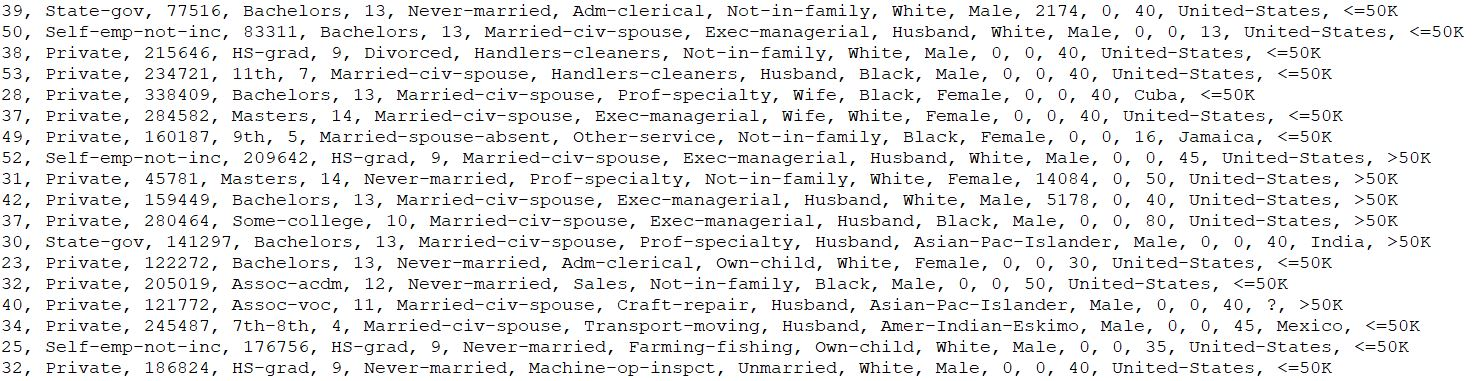
\includegraphics[scale=0.52]{dataset1}
	\caption{Dataset Adults}
	\label{fig:dataset1}
\end{figure}

\noindent Berikut adalah kemungkinan nilai untuk masing-masing jenis atribut dalam dataset:

\begin{itemize}
\item Age: numerik

\item Workclass: Private, Self-emp-not-inc, Self-emp-inc, Federal-gov, Local-gov, State-gov, Without-pay,
Never-worked.

\item Education: Bachelors, Some-college, 11th, HS-grad, Prof-school, Assoc-acdm, Assoc-voc, 9th, 7th-8th, 12th,
Masters, 1st-4th, 10th, Doctorate, 5th-6th, Preschool.

\item Years of education: numerik

\item Marital status: 
Married-civ-spouse, Divorced, Never-married, Separated, Widowed, Married-spouse-absent, MarriedAF-spouse

\item Occupation: Tech-support, Craft-repair, Other-service, Sales, Exec-managerial, Prof-specialty, Handlers-cleaners,
Machine-op-inspect, Adm-clerical, Farming-fishing, Transport-moving, Priv-house-serv, Protective-serv, ArmedForces.

\item Relationship: Wife, Own-child, Husband, Not-in-family, Other-relative, Unmarried

\item Race: White, Asian-Pac-Islander, Amer-Indian-Eskimo, Other, Black

\item Sex: Male, Female

\item Capital gain: numerik

\item Capital loss: numerik

\item Hours per week: numerik

\item Native country: United-States, Cambodia, England, Puerto-Rico, Canada, Germany, Outlying-US(Guam-USVIetc), India, Japan, Greece, South, China, Cuba, Iran, Honduras, Philippines, Italy, Poland, Jamaica, Vietnam, Mexico, Portugal, Ireland, France, Dominican-Republic, Laos, Ecuador, Taiwan, Haiti, Columbia, Hungary, Guatemala, Nicaragua, Scotland, Thailand, Yugoslavia, El-Salvador, Trinidad and Tobago, Peru, Hong, HollandNetherlands

\item Income: $\leq$50K, $>$50K
\end{itemize}


\subsection{Personally Identifiable Information}
Pada bagian \ref{sec:privasi}, telah dijelaskan mengenai konsep Personally Identifiable Information (PII). PII digunakan untuk mengelompokkan nilai atribut berdasarkan kategori atribut yang digunakan pada proses anonimisasi data. Berdasarkan bagian \ref{sec:anonimisasi}, atribut pada proses anonimisasi dapat dikategorikan sebagai identifier, quasi-identifier, dan sensitive attribute. 
\\\\
\noindent Berdasarkan jenis atribut pada dataset Adult, diperoleh kategori sebagai berikut:
\begin{itemize}
\item Identifier (ID): atribut yang nilainya secara langsung dapat mengidentifikasi seseorang\\
Contoh: name (sudah dihilangkan pada dataset)
\item Quasi-identifier (QID): atribut yang nilainya dapat digabungkan dengan atribut lain untuk mengidentifikasi seseorang\\
Contoh: age, zip, education, years of education, occupation, race, sex, native country, income
\item Sensitive Attribute (SA): atribut yang nilainya bersifat privasi atau rahasia\\
Contoh: workclass, marital status, relationship
\end{itemize}

\subsection{Distance, Information Loss, Cost Function}
Distance dan Information Loss digunakan oleh algoritma Greedy K-Member Clustering untuk mencari kelompok data terbaik sehingga menghasilkan pengelompokkan data yang tepat. Cost Function akan dianalisis untuk mencari tahu seberapa baik kinerja algoritma Greedy K-Member Clustering. Cost Function penting untuk dianalisis mengingat data input yang akan diproses berukuran sangat besar.

\subsubsection{Distance}
Distance bertujuan untuk menentukan hasil pengelompokan data pada algoritma Greedy K-Member Clustering. Pemilihan distance yang baik dapat mencapai hasil klasifikasi yang lebih optimal.
\\\\
\noindent Akan diambil 2 sampel data dari dataset Adults sebagai berikut:
\begin{enumerate}
\item 39, State-gov, 77516, Bachelors, 13, Never-married, Adm-clerical, Not-in-family, White, Male, 2174, 0, 40, United-States, <=50K
\item 50, Self-emp-not-inc, 83311, Bachelors, 13, Married-civ-spouse, Exec-managerial, Husband, White, Male, 0, 0, 13, United-States, <=50K
\end{enumerate}

\noindent Distance atribut numerik dapat dihitung sebagai berikut berdasarkan umur data pertama ($v_1$)= 39, umur data kedua ($v_2$)= 50, dan jumlah data ($D$)= 10.000.000 data.


\begin{align*}
\delta_n(v_1,v_2) &= \frac{|v_1 - v_2|}{|D|}
= \frac{|39 - 50|}{10.000.000}\vspace{0.2cm}
= \frac{11}{10.000.000}\vspace{0.2cm}
= 0.0000011
\end{align*}

\noindent Distance atribut kategorikal dapat dihitung sebagai berikut berdasarkan workclass data pertama ($v_1$)= State-gov, workclass data kedua ($v_2$)= Self-emp-not-inc, jumlah subtree ($H(\Lambda(v_i,v_j))$)= 1, dan tinggi taxonomy tree ($H(T_D)$)= 1.

\begin{align*}
\delta_C(v_1,v_2) = \frac{H(\Lambda(v_i,v_j))}{H(T_D)} 
= \frac{1}{1}
= 1
\end{align*}

\begin{figure}[H]
	\centering
	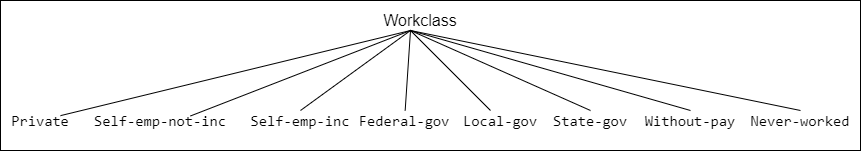
\includegraphics[scale=0.5]{TD}
	\caption{Taxonomy Tree (Workclass)}
	\label{fig:TD}
\end{figure}

\subsubsection{Information Loss}
Information Loss (IL) bertujuan untuk mengevaluasi seberapa baik kinerja algoritma K-Anonymity terhadap utilitas sebuah data. Information Loss (IL) juga dipakai untuk menentukan hasil pengelompokan data pada algoritma Greedy K-Member Clustering. Jika diberikan tabel data yang sudah dikelompokkan berdasarkan cluster, maka nilai Information Loss (IL) dapat dihitung. \\

\newpage
\noindent Berikut adalah contoh hasil pengelompokan data pada cluster 1 untuk dataset Adults:\\

\begin{tabular}{c c c c c c c c}
\hline 
Age & Workclass & Education & Occupation & Sex & Income & Cluster Name \\ 
\hline 
39 & State-gov & Bachelors & Adm-clerical & Male & <=50K & Cluster 1 \\ 

50 & Self-emp-not-inc & Bachelors & Exec-managerial & Male & <=50K & Cluster 1 \\ 

38 & Private & HS-grad & Handlers-cleaners & Male & <=50K & Cluster 1 \\ 

53 & Private & 11th & Handlers-cleaners & Male & <=50K & Cluster 1 \\ 
 
28 & Private & Bachelors & Prof-specialty & Female & <=50K & Cluster 1 \\ 
\hline 
\end{tabular} 

\vspace{0.4cm}

\noindent Information Loss (IL) dapat dihitung sebagai berikut berdasarkan atribut numerik yaitu jumlah anggota cluster ($e$)= 5, $MAX_{Age}$= 53, $MIN_{Age}$= 28, $N_Age$= 5 mencakup atribut Age dan atribut kategorikal yaitu $H(\Lambda(\cup_{C_j}))$= 1, $H(T_{C_j})$= 1 mencakup atribut Workclass, Education, Occupation, Sex, dan Income.

\begin{align*}
D(e) &= \sum_{i=1}^{m} \frac{(MAX_{N_i} - MIN_{N_i})}{|N_i|} + \sum_{j=1}^{n}\frac{H(\Lambda(\cup_{C_j}))}{H(T_{C_j})}\\
&= \frac{(53 - 28)}{5} + \frac{1}{1}+\frac{1}{1}+\frac{1}{1}+\frac{1}{1}+\frac{1}{1} = 10\\\\
IL(e) &= |e| \cdot D(e)\\
&= 5 \cdot 10 = 50
\end{align*}

\noindent Total Information Loss dihitung dari jumlah Information Loss masing-masing cluster.

\begin{align*}
Total-IL(AT) &= \sum_{e \in \varepsilon}^{}  IL(e)\\
&= IL(cluster1)+IL(cluster2)+\ldots+IL(clusterN)
\end{align*}

\subsubsection{Cost Function}
Cost Function bertujuan untuk menghitung kompleksitas algoritma Greedy K-Member Clustering yang sudah dijelaskan pada bagian \ref{sec:greedyclustering}. Kompleksitas akan dianalisis untuk menilai apakah kinerja algoritma sudah sesuai atau belum.\\

\noindent Berikut adalah tahapan kompleksitas dari Algoritma \ref{alg:1} yaitu Find Best Record: 

\begin{enumerate}
\item Baris 5 sampai dengan baris 7, kompleksitasnya 1
\item Baris 8 sampai dengan baris 15, kompleksitasnya n 
\item Kompleksitas totalnya adalah T(n) = 1 + n
\item Algoritma Finding Best Record memiliki kompleksitas O(n)
\end{enumerate}

\noindent Berikut adalah tahapan kompleksitas dari Algoritma \ref{alg:2} yaitu Find Best Cluster:

\begin{enumerate}
\item Baris 5 sampai dengan baris 7, kompleksitasnya 1
\item Baris 8 sampai dengan baris 15, kompleksitasnya n 
\item Kompleksitas totalnya adalah T(n) = 1 + n
\item Algoritma Finding Best Cluster memiliki kompleksitas O(n)
\end{enumerate}

\newpage
\noindent Berikut adalah tahapan kompleksitas dari Algoritma \ref{alg:3} yaitu Greedy K-Member Clustering:

\begin{enumerate}
\item Baris 5 sampai dengan baris 10, kompleksitasnya 1
\item Baris 11 sampai dengan baris 21, kompleksitasnya $n^2$
\item Baris 22 sampai dengan bari 27, kompleksitasnya n
\item Baris 28, kompleksitasnya 1
\item Kompleksitas totalnya adalah T(n) = 1 + $n^2$ + n + 1
\item Algoritma Finding Best Cluster memiliki kompleksitas O($n^2$)
\end{enumerate}

\subsection{Greedy K-Member Clustering}
Algoritma Greedy K-Member Clustering bertujuan untuk membagi seluruh data pada tabel terhadap masing-masing cluster untuk kompleksitas yang lebih baik dan mendukung nilai utilitas informasi yang lebih baik dibandingkan algoritma clustering lain. Pada bagian ini, akan dilakukan eksperimen sederhana mengenai algoritma Greedy K-Member Clustering terhadap dataset Adults untuk mencari tahu langkah kerja algoritma Greedy K-Member Clustering secara konseptual. \\

\noindent Diberikan contoh sampel dataset Adults sebagai berikut:
\\\\
\begin{tabular}{c c c c c c c c}
\hline 
ID & Age & Workclass & Education & Occupation & Sex & Income\\ 
\hline 
t1 & 39 & State-gov & Bachelors & Adm-clerical & Male & <=50K \\ 

t2 & 50 & Self-emp-not-inc & Bachelors & Exec-managerial & Male & <=50K  \\ 

t3 & 38 & Private & HS-grad & Handlers-cleaners & Male & <=50K  \\ 

t4 & 53 & Private & 11th & Handlers-cleaners & Male & <=50K  \\ 
 
t5 & 28 & Private & Bachelors & Prof-specialty & Female & <=50K	 \\ 
\hline 
\end{tabular} 
\\\\
\par Melalui sampel data pada tabel 2.1, akan diputuskan nilai dari setiap atribut anonimisasi. Jenis atribut anonimisasi yang pertama adalah Quasi-identifier, dengan nilai QI = \{Age, Education, Occupation, Sex, Income\}. Jenis atribut anonimisasi yang kedua adalah Sensitive Attribute, dengan nilai SA = \{Workclass\}. Jika telah diketahui tabel data seperti diatas, k = 2, dan jumlah cluster (m) = 2, maka algoritma Greedy K-Member Clustering siap ditelusuri lebih lanjut.\\

\noindent Berikut adalah tahapan yang terjadi pada algoritma Greedy K-Member Clustering:

\begin{enumerate}
\item Nilai awal result = $\emptyset$
\item Nilai awal r = \{t1\}
\item Nilai awal |S| = 5, k = 2
\item Karena kondisi $|S| \geq k$ terpenuhi, maka dilakukan perulangan sebagai berikut:
\begin{enumerate}
\item Nilai r diubah menjadi r = \{t3\}, karena terbukti data t3 memiliki $\Delta(t1,t3)=1.7189$ yang paling tinggi dari seluruh distance lain. Berikut adalah contoh perhitungannya:
\begin{align*}
\Delta (t_1,t_2) = 1.715\\
\Delta (t_1,t_3) = 2.431\\
\Delta (t_1,t_4) = 2.122\\
\Delta (t_1,t_5) = 1.621 
\end{align*}
\item Nilai awal S = \{t1, t2, t4, t5\}
\item Nilai awal c = \{t3\}, |c| = 1
\item Karena kondisi |c| < k terpenuhi, maka dilakukan perulangan sebagai berikut:

\begin{enumerate}
\item Nilai r diubah menjadi r = \{t3,t4\}, karena terbukti data t4 memiliki $IL(t3 \cup t4)=0.330$ yang paling rendah dari seluruh data lain. Berikut adalah contoh perhitungannya:
\begin{align*}
IL(t3 \cup t1) = 0.479 \\
IL(t3 \cup t2) = 0.515 \\
IL(t3 \cup t4) = 0.330 \\
IL(t3 \cup t5) = 0.367 
\end{align*}
\item Nilai S diubah menjadi S = \{t1, t2, t5\}, |S| = 4
\item Nilai c ditambahkan menjadi c = \{t3, t4\}, |c| = 2

\end{enumerate}
\item Karena kondisi |c| < k sudah tidak terpenuhi lagi, maka perulangan ini akan berhenti
\item Nilai result akan ditambahkan menjadi result = \{t3, t4\}
\item Karena kondisi $|S| \geq k$ masih terpenuhi, maka perulangan akan tetap berlanjut sampai pada kondisi dimana $|S| < k$ sehingga hasil akhirnya adalah result = \{\{t3, t4\}, \{t2, t5\}\}, S = \{t1\}, |S| = 1

\end{enumerate}

\item Karena kondisi $S \neq 0$ terpenuhi, maka dilakukan perulangan sebagai berikut:

\begin{enumerate}
\item Nilai r diubah menjadi r = \{t1\}
\item Nilai S diubah menjadi S = $\{\phi\}$, |S| = 0
\item Nilai c diubah menjadi c = \{t3, t4\} karena terbukti cluster c memiliki $IL(\{t3,t4\} \cup t1)=0.279$ yang paling rendah dari seluruh cluster lain. Berikut adalah contoh perhitungannya:
\begin{align*}
IL(\{t3,t4\} \cup t1) = 0.279 \\
IL(\{t2,t5\}\cup t1) = 0.515 \\
\end{align*}
\item Nilai c ditambahkan menjadi c = \{t1, t3, t4\}
\item Nilai c pada perulangan ini tidak akan ditambahkan pada result, karena telah ditetapkan k = 2 sedangkan jumlah datanya ganjil, sehingga sisa data tersebut tidak akan dicatat pada result agar menjaga masing-masing cluster hanya memiliki 2 anggota saja.
\item Karena kondisi $S \neq 0$ sudah tidak terpenuhi lagi, maka perulangan ini akan berhenti

\end{enumerate}

\item Hasil akhirnya adalah result = \{\{t3, t4\}, \{t2, t5\}\} dikembalikan sebagai output untuk algoritma Greedy K-Member Clustering seperti pada tabel berikut:\\

\begin{tabular}{c c c c c c c c}
\hline 
ID & Age & Workclass & Education & Occupation & Sex & Income\\ 
\hline 
t3 & 38 & Private & HS-grad & Handlers-cleaners & Male & <=50K  \\ 
t4 & 53 & Private & 11th & Handlers-cleaners & Male & <=50K  \\ 
\hline 
t2 & 50 & Self-emp-not-inc & Bachelors & Exec-managerial & Male & <=50K  \\ 
t5 & 28 & Private & Bachelors & Prof-specialty & Female & <=50K	 \\ 
\hline 
\end{tabular} 

\end{enumerate}

\subsection{Domain Generalization Hierarchy}
Domain Generalization Hierarychy (DGH) bertujuan untuk melindungi data dengan cara menerapkan metode generalisasi terhadap nilai atribut data yang bersifat unik, agar menjadi nilai yang lebih umum. Nilai yang lebih umum biasa sulit untuk ditebak karena mengandung beberapa arti dalam satu nilai, berbeda dengan nilai yang bersifat unik yang memiliki satu arti dalam satu nilai. Pada bagian ini, akan dilakukan eksperimen sederhana mengenai penerapan DGH terhadap masing-masing atribut pada dataset Adults, untuk mencari tahu langkah kerja DGH secara konseptual. \\

\noindent Diketahui kemungkinan nilai atribut numerik pada dataset Adults adalah sebagai berikut:

\begin{itemize}
\item Age = \{33,36,38,40,42,43,46,49\}
\item ZIP = \{77516,77517,77526,77527\}
\item Sex = \{Male,Female\}
\item Hours/week = \{12,18,33,37,53,54\}
\end{itemize}

\noindent Berikut adalah tahapan yang terjadi pada Domain Generalization Hierarchy:

\begin{enumerate}
\item Dipilih atribut quasi-identifier sebagai berikut QI = \{Age, ZIP, Sex, Hours per week\}
\item Diketahui domain dasar dari atribut ZIP yaitu $Z_0$ = \{77516,77517,77526,77527\}
\item Membuat domain yang kurang spesifik berdasarkan tiga cara:
\begin{itemize}
\item Untuk atribut numerik dengan jumlah digit < 2, maka hasilnya sebagai berikut jika atributnya Age, $Z_1$ = \{[33-38],[40-49]\} 
\item Untuk atribut numerik  dengan jumlah digit > 2, maka hasilnya sebagai berikut jika atributnya ZIP, $Z_1$ = \{7751*,7752*\}
\item Untuk atribut kategorikal, maka hasilnya adalah nilai yang lebih umum sebagai berikut jika atributnya Sex, $Z_1$ = \{Person\}
\end{itemize} 
\item Membuat domain yang lebih umum dari atribut ZIP yaitu $Z_2$ = \{775**\}
\item Membuat domain yang sangat umum dari atribut ZIP yaitu $Z_3$ = \{*****\}
\item Memilih domain sesuai kebutuhan, biasanya dipilih domain yang kurang spesifik seperti $Z_1$ = \{7751*,7752*\} atau domain yang lebih umum seperti $Z_2$ = \{775**\}
\item Langkah ini diulangi sampai seluruh atribut quasi-identifier telah selesai digeneralisasi.
\item Hasil akhir dari DGH adalah sebagai berikut: 
\begin{align*}
Age &= \{[33-38], [40-49]\}\\
ZIP &= \{7751*, 7752*\}\\
Sex &= \{Person\}\\
Hours/Week &=\{[12-18], [33-37], [53-54]\}
\end{align*} 
\item Proses generalisasi DGH telah selesai dilakukan. Tahap selanjutnya adalah proses anonimisasi data pada tabel dataset.
\end{enumerate}



\subsection{Anonimisasi}
Anonimisasi bertujuan untuk menyamarkan nilai dari masing quasi-identifier yang unik pada kelompok cluster yang sama. Kata kuncinya adalah nilai unik pada kelompok cluster yang sama. Setelah dataset dilakukan anonimisasi, maka data privasi secara konseptual sudah terlindungi sehingga publikasi data dapat dilakukan dengan aman.
\\\\
\noindent Diketahui kelompok data berdasarkan algoritma Greedy K-Member Clustering sebagai berikut: \\

\begin{tabular}{c c c c c c c c}
\hline 
ID & Age & Workclass & Education & ZIP & Sex & Hours/week & Cluster Name\\ 
\hline 
t3 & 32 & Private & HS-grad & 77516 & Male & 30 & Cluster 1 \\ 
t4 & 32 & Private & 11th & 77541 & Female & 30 & Cluster 1 \\ 
\hline 
t2 & 34 & Self-emp-not-inc & Bachelors & 77526 & Male & 34 & Cluster 2 \\ 
t5 & 50 & Private & Bachelors & 77526 & Male & 37	& Cluster 2\\ 
\hline 
t1 & 47 & Local-gov & Bachelors & 77581 & Male & 54 & Cluster 3\\ 
t6 & 50 & Federal-gov & HS-grad & 77532 & Male & 57 & Cluster 3\\ 
\hline 
\end{tabular} 

\vspace{0.4cm}

\noindent Diketahui bentuk generalisasi berdasarkan Domain Generalization Hierarchy sebagai berikut:
\begin{align*}
Age &= \{[20-30], [40-50]\}\\
ZIP &= \{775**\}\\
Sex &= \{Person\}\\
Hours/week &=\{[12-18], [33-37], [53-61]\}
\end{align*} 

\noindent Berikut adalah tahapan yang terjadi pada proses anonimisasi:
\begin{enumerate}

\item Diketahui Quasi-Identifier sebagai berikut QI = \{Age, ZIP, Sex, Hours/week\} dan sensitive attribute sebagai berikut SA = \{Workclass, Education\}

\item Mencari nilai Quasi-Identifier yang unik pada kelompok cluster yang sama. Sebagai contoh, cluster 2 memiliki nilai quasi-identifier yang unik sebagai berikut QI = \{Age, Hours/week\}

\item Melakukan generalisasi DGH pada nilai quasi-identifier yang unik menjadi bentuk . Sebagai contoh, QI = \{Age, Hours/week\} memiliki nilai yang unik, sehingga diubah menjadi Age = \{[40-50]\}, Hours/week = \{[33-37]\}

\item Sensitive Attribute tidak akan dilakukan generalisasi, karena Quasi-Identifier sudah dilakukan generalisasi sehingga seseorang akan sulit untuk menebak kepemilikan dari Sensitive Attribute.

\item Ulangi hal yang sama pada langkah sebelumnya untuk setiap cluster. Hasil akhir dari tabel dataset setelah dianonimisasi adalah sebagai berikut:  \\

\begin{tabular}{c c c c c c c c}
\hline 
ID & Age & Workclass & Education & ZIP & Sex & Hours/week & Cluster Name\\ 
\hline 
t3 & 32 & Private & HS-grad & 775** & Person & 30 & Cluster 1 \\ 
t4 & 32 & Private & 11th & 775** & Person & 30 & Cluster 1 \\ 
\hline 
t2 & [40-50] & Self-emp-not-inc & Bachelors & 77526 & Male & [33-37] & Cluster 2 \\ 
t5 & [40-50] & Private & Bachelors & 77526 & Male & [33-37]	& Cluster 2\\ 
\hline 
t1 & [40-50] & Local-gov & Bachelors & 775** & Male & [53-61] & Cluster 3\\ 
t6 & [40-50] & Federal-gov & HS-grad & 775** & Male & [53-61] & Cluster 3\\ 
\hline 
\end{tabular} 

\item Proses anonimisasi data telah selesai dilakukan. Pada tahap ini dataset telah aman untuk dilakukan publikasi data.

\end{enumerate}

\section{Eksplorasi Spark}
Pada bagian ini akan dilakukan penelusuran lebih lanjut mengenai beberapa hal penting terkait Spark sebelum melakukan eksperimen metode anonimisasi pada Spark.\\ 

\noindent Berikut adalah beberapa hal penting terkait Spark:
\begin{itemize}

\item Spark bekerja sama dengan komponen lain seperti JDK, SBT, HDFS sehingga instalasi Spark untuk masing-masing sistem operasi dapat berbeda. Pada penelitian in, akan dilakukan instalasi Spark melalui sistem operasi Windows. 

\item Spark dapat bekerja dengan bahasa pemrograman Scala. Scala dipilih karena memiliki efektivitas yang baik pada penulisan kode program. Scala dapat menyederhanakan perintah pada Spark menjadi baris yang lebih sedikit.

\item Program Spark dijalankan dengan cara membuat jar sebelum perintah eksekusi dijalankan. Hal ini menghambat perkerjaan pada tahap implementasi perangkat lunak. Intel IJ adalah sebuah Integrated Development Environment (IDE) yang memfasilitasi pemrograman Scala pada Spark dan menampilkan hasil pemrosesan Spark  secara langsung.

\item Spark menyediakan konfigurasi untuk mengatur jumlah resource  yang dibutuhkan (jumlah pemakaian RAM, core CPU) pada pemrosesan data. Konfigurasi ini bertujuan agar Spark dapat mengolah data yang besar secara maksimal dengan menggunakan jumlah resource yang tersedia. Konfigurasi ini ditulis pada perintah eksekusi Spark.
 

\end{itemize}



\subsection{Instalasi Spark}
Spark dapat berjalan pada sistem operasi Windows, Linux, dan Mac OS. Spark dapat dijalankan secara lokal menggunakan satu komputer, meskipun nyatanya Spark tetap membutuhkan beberapa komputer agar pemrosesan data yang besar dapat menjadi lebih cepat. Pada bagian ini akan dijelaskan tahapan instalasi Spark untuk versi 2.4.5 pada sistem operasi Windows dari awal hingga akhir. Sebelum melakukan instalasi Spark, ada beberapa hal yang harus diperhatikan dan dipenuhi. 
\\\\
\noindent Berikut adalah beberapa hal yang harus diperhatikan:

\begin{itemize}
\item Java 7, Python 2.6 telah dihilangkan pada implementasi Spark 2.2.0
\item Scala 2.10 sudah tidak dapat dipakai, Scala 2.11 sudah terlalu usang untuk dipakai pada Spark 2.4.1 dan akan dihilangkan pada Spark 3.0
\item Hadoop 2.6.5 telah dihilangkan pada implementasi Spark 2.2.0 
\end{itemize}

\noindent Berikut adalah beberapa hal yang harus dipenuhi:

\begin{itemize}
\item Spark 2.4.5 berjalan di Java 8, Python 2.7+/3.4+ dan R 3.1+ 
\item Spark 2.4.5 menggunakan Scala 2.12
\item Spark 2.4.5 menggunakan Hadoop 2.7
\end{itemize}

\noindent Berikut adalah tahapan instalasi Spark 2.4.5 secara umum:

\begin{enumerate}
\item Melakukan instalasi Java 8.
\item Melakukan instalasi Spark 2.4.5
\item Melakukan instalasi IntelIJ untuk Scala sbt.
\end{enumerate}

\newpage
\subsubsection{Instalasi Java 8}
\noindent Berikut adalah tahapan instalasi Java 8 secara lengkap:

\begin{enumerate}

\item Download Java SE Development Kit 8u31 pada link berikut \path{https://www.oracle.com/technetwork/java/javase/downloads/java-archive-javase8-2177648.html}
 
\item Lakukan instalasi Java SE Development Kit 8u31 seperti biasa.

\item Pilih menu Edit the system environment variables.

\item Buat environment variables baru seperti gambar berikut.

\begin{figure}[H]
	\centering
	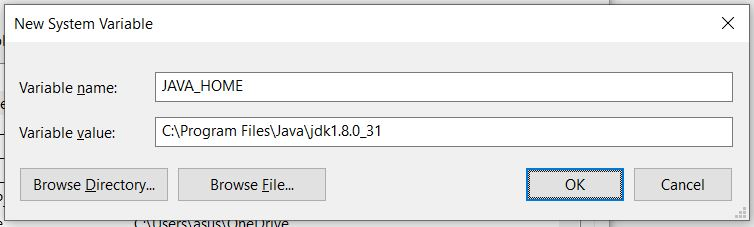
\includegraphics[scale=0.7]{instal_java_5}
	\caption{Environment Variables}
	\label{fig:instal_java_5}
\end{figure}


\item Tambahkan \path{%JAVA_HOME%\bin;} pada Path di System variables

\begin{figure}[H]
	\centering
	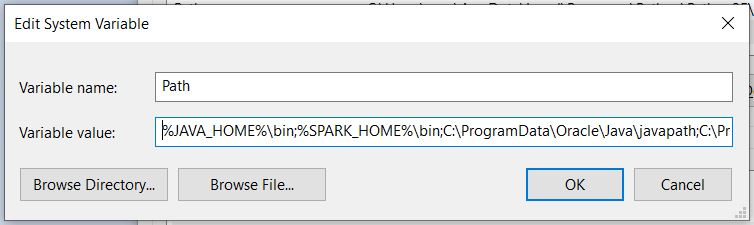
\includegraphics[scale=0.8]{spark_instal_5}
	\caption{Penambahan Variable Value}
	\label{fig:spark_instal_5}
\end{figure}

\item Pada tahap ini Java 8 sudah terpasang, langkah selanjutnya adalah melakukan verifikasi instalasi untuk memeriksa apakah instalasi tersebut dapat berjalan dengan baik.

\end{enumerate}

\noindent Berikut adalah tahapan verifikasi terhadap instalasi Java 8:

\begin{enumerate}

\item Pilih menu Command Prompt.

\item Jalankan perintah java -version pada Command Prompt.

\item Apabila sistem tidak menampilkan pesan error, maka Java 8 sudah terpasang dengan baik.

\end{enumerate}

\newpage
\subsubsection{Instalasi Spark 2.4.5}
Berikut adalah tahapan instalasi Spark 2.4.5 secara lengkap:
\begin{enumerate}

\item Download winutils.exe dari link \path{https://github.com/steveloughran/winutils/tree/master/hadoop-2.7.1/bin}

\item Buat folder seperti berikut \path{C:\winutils\bin} dan tempatkan winutils.exe di dalam folder tesebut.

\item Download Spark 2.4.5 dari link \path{https://downloads.apache.org/spark/spark-3.0.0-preview2/spark-3.0.0-preview2-bin-hadoop2.7.tgz}

\item Buat folder sebagai berikut \path{C:\spark-2.4.4} dan ekstraksi  file \path{spark-2.4.5-bin-hadoop2.7.tgz} di dalam folder tersebut.

\item Pilih menu Edit the system environment variables

\item Buat environment variables baru seperti gambar berikut.

\begin{figure}[H]
	\centering
	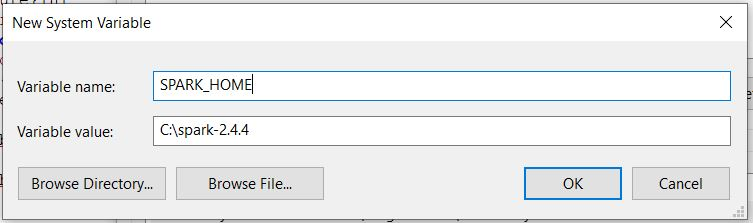
\includegraphics[scale=0.45]{spark_instal_3}
	\caption{Environment Variable}
	\label{fig:spark_instal_3}
\end{figure}

\item Tambahkan \path{%SPARK_HOME%\bin;} pada Path di System variables

\begin{figure}[H]
	\centering
	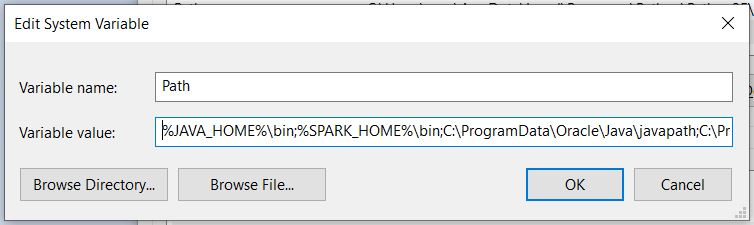
\includegraphics[scale=0.45]{spark_instal_5}
	\caption{Penambahan Variable Value}
	\label{fig:spark_instal_5}
\end{figure}

\item Pada tahap ini Spark 2.4.5 sudah terpasang, langkah selanjutnya adalah melakukan verifikasi instalasi untuk memeriksa apakah instalasi tersebut dapat berjalan dengan baik.

\end{enumerate}

\noindent Berikut adalah tahapan verifikasi terhadap instalasi Spark 2.4.5:
\begin{enumerate}
\item Jalankan perintah \path{spark-shell} pada Command Prompt.

\item Apabila tampilan berubah seperti gambar berikut, artinya Spark 2.4.5 sudah dapat berjalan dengan baik.

\begin{figure}[H]
	\centering
	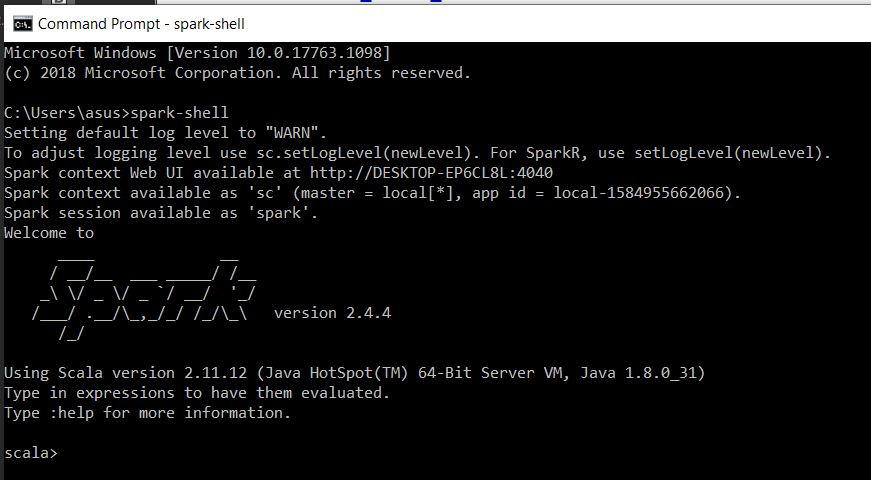
\includegraphics[scale=0.40]{spark_instal_7}
	\caption{Spark 2.4.5}
	\label{fig:spark_instal_7}
\end{figure}

\end{enumerate}

\newpage
\subsubsection{Instalasi IntelIJ untuk Scala}
Berikut adalah tahapan instalasi IntelIJ:

\begin{enumerate}
\item Download IntelIJ melalui link berikut \path{https://www.jetbrains.com/idea/download/#section=windows}

\item Lakukan instalasi IntelIJ seperti biasa.

\item Pada tahap ini IntelIJ sudah terpasang dengan baik pada komputer, langkah selanjutnya adalah melakukan instalasi plugin Scala pada IntelIJ.

\end{enumerate}

\noindent Berikut adalah tahapan pemasangan plugin Scala pada IntelIJ.

\begin{enumerate}

\item Pilih menu Configure pada IntelIJ, lalu pilih menu Plugins.

\item Telusuri plugins Scala pada kolom pencarian.
\begin{figure}[H]
	\centering
	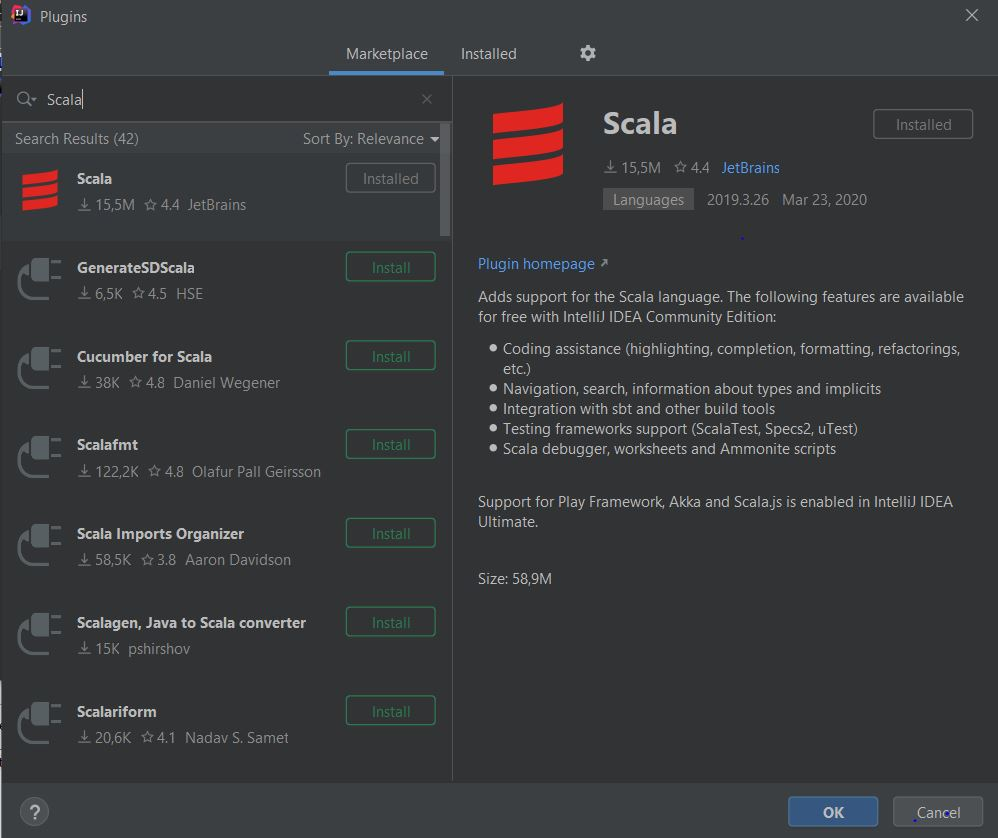
\includegraphics[scale=0.50]{intelij_2}
	\caption{Plugins Scala}
	\label{fig:intelij_2}
\end{figure}

\item Klik tombol install

\item Pada tahap ini program Spark sudah dapat berjalan dan dikompilasi dengan IntelIJ, langkah selanjutnya adalah membuat project Spark baru pada IntelIJ.

\end{enumerate}


\newpage
\subsection{Membuat Project Spark pada IntelIJ}
Untuk membuat program Spark, pertama-tam perlu membuat project Spark baru untuk merancang kelas-kelas yang dibutuhkan pada eksekusi Spark. Beberapa hal yang perlu diperhatikan adalah menggunakan versi Scala sbt, memilih versi sbt 1.3.9, memilih versi Scala 2.11.12, dan melakukan import libraryDependencies Spark sesuai kebutuhan.\\

\noindent Berikut adalah tahapan pembuatan project Spark pada IntelIJ:

\begin{enumerate}
\item Memilih menu Create New Project

\item Menggunakan bahasa pemrograman Scala dengan berbasis sbt.
\begin{figure}[H]
	\centering
	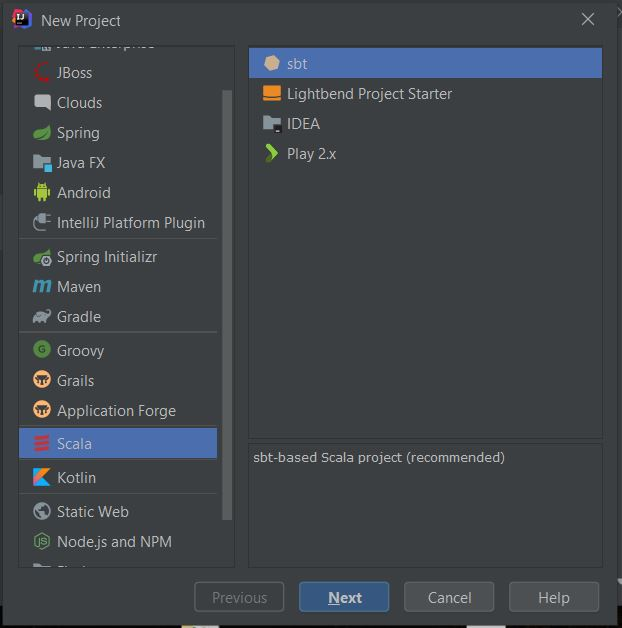
\includegraphics[scale=0.58]{proyeksparksederhana1.JPG}
	\caption{Plugins Scala}
	\label{fig:proyeksparksederhana1.JPG}
\end{figure}

\item Melakukan konfigurasi pada project Spark baru
\begin{figure}[H]
	\centering
	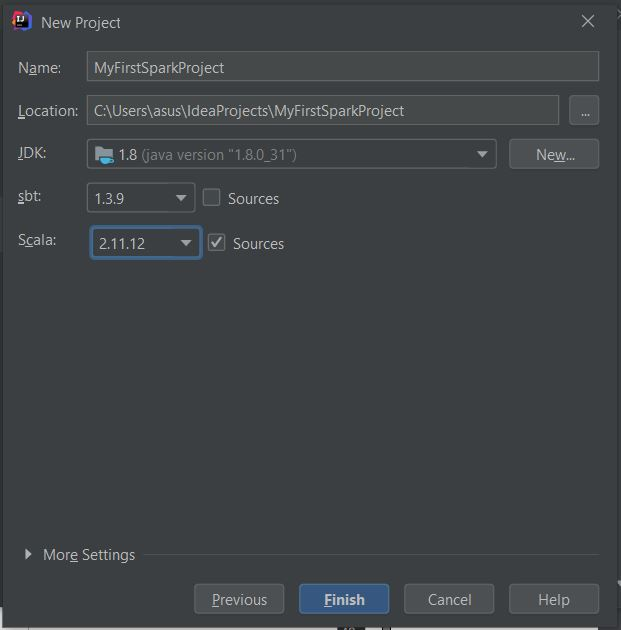
\includegraphics[scale=0.58]{proyeksparksederhana2.JPG}
	\caption{Plugins Scala}
	\label{fig:proyeksparksederhana2.JPG}
\end{figure}

\item Melakukan import libraryDependencies sesuai kebutuhan pada file \path{build.sbt} \\ 
Contoh: spark-core, spark-sql, spark-mllib.
\begin{lstlisting}[basicstyle=\ttfamily, frame=single,
	columns=fullflexible, keepspaces=true, breaklines=true, label=ls_kepatuhan_1_1_1_logo_sharif_judge, caption=Main method]
name := "NamaProject"
version := "0.1"
scalaVersion := "2.11.12"
// https://mvnrepository.com/artifact/org.apache.spark/spark-core
libraryDependencies += "org.apache.spark" %% "spark-core" % "2.2.0"
// https://mvnrepository.com/artifact/org.apache.spark/spark-sql
libraryDependencies += "org.apache.spark" %% "spark-sql" % "2.4.0"
// https://mvnrepository.com/artifact/org.apache.spark/spark-mllib
libraryDependencies += "org.apache.spark" %% "spark-mllib" % "2.4.3"

\end{lstlisting}

\item Menambahkan Scala class pada \path{src/main/scala}.  
\begin{figure}[H]
	\centering
	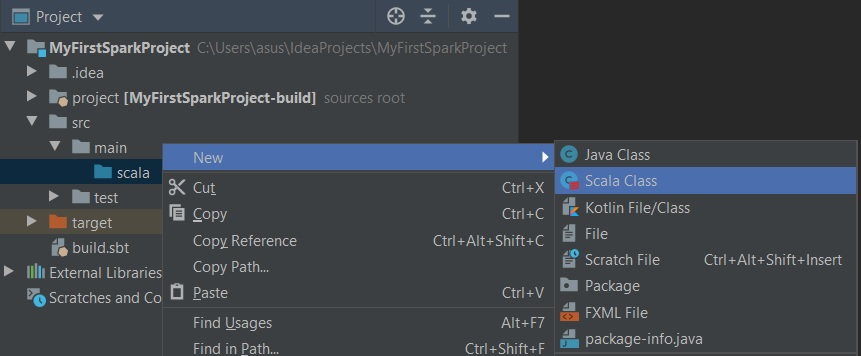
\includegraphics[scale=0.7]{proyeksparksederhana5.JPG}
	\caption{Plugins Scala}
	\label{fig:proyeksparksederhana5.JPG}
\end{figure}

\item Memilih tipe Scala class sebagai Object.
\begin{figure}[H]
	\centering
	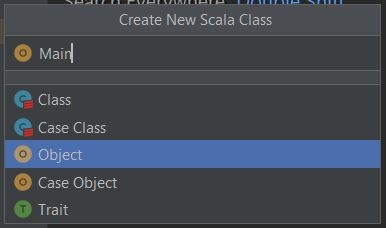
\includegraphics[scale=0.8]{proyeksparksederhana6.JPG}
	\caption{Plugins Scala}
	\label{fig:proyeksparksederhana6.JPG}
\end{figure}

\item Menambahkan main method pada Scala class.
\begin{lstlisting}[basicstyle=\ttfamily, frame=single,
	columns=fullflexible, keepspaces=true, breaklines=true, label=ls_kepatuhan_1_1_1_logo_sharif_judge, caption=Main method]
object Main {
  def main(args: Array[String]) {
  	 //statement		
  }
}
\end{lstlisting}



\end{enumerate}

\subsection{Membuat File JAR pada Command Prompt}
Sebelum menjalankan program Spark pada Hadoop Cluster, program Spark yang sudah jadi harus dibuat menjadi file JAR terlebih dahulu. Hal ini disebabkan karena perintah Spark hanya menerima input berupa kode program dalam format (.jar).\\

\noindent Berikut adalah tahapan untuk membuat JAR:
\begin{enumerate}
\item Membuka folder pengerjaan project Spark \path{\IdeaProjects\NamaProject}
\item Membuka command prompt pada folder project.
\item Mengeksekusi perintah \textsf{sbt package} pada command prompt
\item Menunggu proses pembuatan file JAR oleh sistem, apabila terminal tidak menampilkan pesan error maka file JAR telah berhasil dibuat dan tersimpan pada folder tertentu.
\item File JAR yang telah dibuat akan tersimpan pada \path{NamaProject\target\scala-2.11} 
\end{enumerate}

\subsection{Menjalankan Program Spark pada Command Prompt}
Apabila ukuran data input eksperimen kecil, maka program Spark dapat dijalankan pada komputer lokal menggunakan perintah dari Command Prompt. \\

\noindent Berikut adalah tahapan menjalankan program Spark pada Command Prompt:
\begin{enumerate}
\item Membuka command prompt pada komputer lokal.
\item Menjalankan perintah eksekusi Spark sebagai berikut \textsf{spark-submit --class NamaMainClass --master local[*] \path{lokasi_jar\nama_jar.jar}} pada command prompt
\item Menunggu proses eksekusi file JAR oleh komputer lokal, apabila terminal tidak menampilkan pesan error maka program Spark berhasil dijalankan dengan baik.
\end{enumerate}

\subsection{Menjalankan Program Spark pada Hadoop Cluster}
Karena ukuran data input eksperimen terbilang besar yaitu mencapai 1GB, maka akan lebih efektif apabila komputasi dilakukan secara paralel melalui Hadoop cluster. Hadoop cluster terdiri dari beberapa perangkat komputer yang dapat saling bekerja sama, sehingga proses komputasi dapat dilakukan lebih cepat.\\

\noindent Berikut adalah tahapan menjalankan program Spark pada Hadoop cluster:
\begin{enumerate}
\item Membuka command prompt pada komputer lokal.
\item Menyambungkan jaringan komputer lokal dengan server Hadoop cluster menggunakan perintah \textsf{ssh hduser@10.100.69.101} pada command prompt.
\item Melakukan upload file JAR dari komputer lokal ke folder Hadoop cluster menggunakan perintah \textsf{scp \path{nama_jar.jar} hduser
$@$10.100.69.101:\path{nama_folder}} pada command prompt.
\item Menjalankan perintah eksekusi Spark sebagai berikut \textsf{spark-submit --class NamaMainClass --master yarn \path{lokasi_jar\nama_jar.jar}} pada command prompt
\item Menunggu proses eksekusi file JAR oleh Hadoop cluster, apabila terminal tidak menampilkan pesan error maka program Spark berhasil dijalankan dengan baik.
\end{enumerate}

\newpage
\section{Studi Kasus}
Untuk memahami implementasi algoritma anonimisasi pada Spark, maka dilakukan studi kasus terhadap fungsi Spark yang umum digunakan, seperti fungsi dasar pada Spark, fungsi dasar pada komponen Spark, dan fungsi dasar pada Spark MLlib. Bentuk dari studi kasus yang akan dilakukan adalah memberikan contoh kode program berikut penjelasan singkat mengenai tujuan pemanggilan fungsi, parameter input, dan contoh output yang dikeluarkan oleh fungsi tersebut.

\subsection{Eksperimen Scala}

\subsubsection{Menentukan Jenis Variabel pada Scala}
Scala memiliki dua jenis varibel yaitu immutable variabel dan mutable variabel. Immutable variabel adalah variabel yang nilainya tidak dapat diubah, sedangkan mutable variabel adalah variabel yang nilainya dapat diubah. Implementasi immutable dan mutable memiliki implementasi sintaks yang berbeda. Immutable variabel menggunakan sintaks val, sedangkan mutable variabel menggunakan sintaks var. Kode program pada bagian ini dapat dilihat pada Listing \ref{lst:jenis_variabel} mengenai jenis variabel pada Scala.

\begin{lstlisting}[basicstyle=\ttfamily, frame=single,
	columns=fullflexible, keepspaces=true, breaklines=true, label=lst:jenis_variabel, caption=Menentukan Jenis Variabel pada Scala]
	
// Immutable Variabel
val donutsToBuy: Int = 5
donutsToBuy = 10

// Mutable Variabel
var favoriteDonut: String = "Glazed Donut"
favoriteDonut = "Vanilla Donut"


\end{lstlisting}

\subsubsection{Menentukan Jenis Tipe Data pada Scala}
Scala memiliki jenis tipe data yang mirip dengan tipe data pada bahasa pemrograman Java. Scala dapat menangani tipe data Int, Long, Short, Double, Float, String, Byte, Char dan Unit. Kode program pada bagian ini dapat dilihat pada Listing \ref{lst:jenis_tipe_data} mengenai jenis tipe data pada Scala.

\begin{lstlisting}[basicstyle=\ttfamily, frame=single,
	columns=fullflexible, keepspaces=true, breaklines=true, label=lst:jenis_tipe_data, caption=Menentukan Jenis Tipe Data pada Scala]
	
val donutsBought: Int = 5
val bigNumberOfDonuts: Long = 100000000L
val smallNumberOfDonuts: Short = 1
val priceOfDonut: Double = 2.50
val donutPrice: Float = 2.50f
val donutStoreName: String = "allaboutscala Donut Store"
val donutByte: Byte = 0xa
val donutFirstLetter: Char = 'D'
val nothing: Unit = ()

\end{lstlisting}

\newpage
\subsubsection{Menentukan Struktur Data pada Scala}
Scala memiliki dua jenis struktur data yaitu immutable dan mutable collection. Immutable collection adalah struktur data yang nilainya tidak dapat diubah, sedangkan mutable collection adalah struktur data yang nilainya dapat diubah. Implementasi immutable dan mutable collection memiliki jenis struktur data yang berbeda satu sama lain. Kode program pada bagian ini dapat dilihat pada Listing \ref{lst:immutable_collection} mengenai immutable collection pada Scala dan Listing \ref{lst:mutable_collection} mengenai  mutable collection pada Scala.

\begin{lstlisting}[basicstyle=\ttfamily, frame=single,
	columns=fullflexible, keepspaces=true, breaklines=true, label=lst:immutable_collection, caption=Membuat immutable collection pada Scala]
	
// List
val list1: List[String] = List("Plain Donut","Strawberry Donut","Chocolate Donut")
println(s"Elements of list1 = $list1")

// Map
val map1: Map[String, String] = Map(("PD","Plain Donut"),("SD","Strawberry Donut"),("CD","Chocolate Donut"))
println(s"Elements of map1 = $map1")

\end{lstlisting}

\begin{lstlisting}[basicstyle=\ttfamily, frame=single,
	columns=fullflexible, keepspaces=true, breaklines=true, label=lst:mutable_collection, caption=Membuat mutable collection pada Scala]
	
// Array
val array1: Array[String] = Array("Plain Donut","Strawberry Donut","Chocolate Donut")
println(s"Elements of array1 = ${array1.mkString(", ")}")

// Map
val map1: Map[String, String] = Map(("PD","Plain Donut"),("SD","Strawberry Donut"),("CD","Chocolate Donut"))
println(s"Elements of map1 = $map1")

\end{lstlisting}

\subsubsection{Membuat Kelas Object pada Scala}
Scala menggunakan kelas Object untuk menempatkan berbagai macam fungsi dan variabel yang saling berkaitan pada satu kelas yang sama. Kode program pada bagian ini dapat dilihat pada Listing \ref{lst:kelas_object} mengenai kelas object pada Scala.

\begin{lstlisting}[basicstyle=\ttfamily, frame=single,
	columns=fullflexible, keepspaces=true, breaklines=true, label=lst:kelas_object, caption=Membuat Kelas Object pada Scala]
	
object DonutShoppingCartCalculator {

 val discount: Double = 0.01

 def calculateTotalCost(donuts: List[String]): Double = {
  // calculate the cost of donuts
  return 1
 }
 
}
	
\end{lstlisting}

\newpage
\subsubsection{Membuat Fungsi Sederhana pada Scala}
Scala menggunakan fungsi untuk menempatkan kode program berdasarkan tujuan masing-masing. Perlu diperhatikan bahwa hasil akhir dari fungsi langsung dikembalikan tanpa memanggil perintah return, seperti pada Java. Kode program pada bagian ini dapat dilihat pada Listing \ref{lst:fungsi_sederhana} mengenai pembuatan fungsi pada Scala.

\begin{lstlisting}[basicstyle=\ttfamily, frame=single,
	columns=fullflexible, keepspaces=true, breaklines=true, label=lst:fungsi_sederhana, caption=Membuat Fungsi Sedehana pada Scala]
	
def calculateDonutCost(donutName: String, quantity: Int): Double = {
  println(s"Calculating cost for $donutName, quantity = $quantity")

  // make some calculations ...
  2.50 * quantity
}
	
\end{lstlisting}


\subsubsection{Membuat Main Method}
Scala menggunakan main method untuk melakukan eksekusi program. Kode program pada bagian ini dapat dilihat pada Listing \ref{lst:main_method} mengenai pembuatan main method pada Scala.

\begin{lstlisting}[basicstyle=\ttfamily, frame=single,
	columns=fullflexible, keepspaces=true, breaklines=true, label=lst:main_method, caption=Membuat Main Method pada Scala]
	
object HelloWorld {
	def main(args: Array[String] {
		println("Hellow, world!")
	}
}
	
\end{lstlisting}

\subsubsection{Membuat Fungsi Percabangan}
Scala memiliki jenis implementasi percabangan yang sama dengan Java. Percabangan digunakan untuk melakukan eksekusi pada baris statement yang sesuai berdasarkan kondisi tertentu. Kode program pada bagian ini dapat dilihat pada Listing \ref{lst:percabangan} mengenai percabangan pada Scala.

\begin{lstlisting}[basicstyle=\ttfamily, frame=single,
	columns=fullflexible, keepspaces=true, breaklines=true, label=lst:percabangan, caption=Membuat Fungsi Percabangan pada Scala]

# If-Else statement
if(numberOfPeople > 10) { 
  println(s"Number of donuts to buy = ${numberOfPeople * donutsPerPerson}")
}
else if (numberOfPeople == 0) {
  println("Number of people is zero.")
  println("No need to buy donuts.")
} 
else {
  println(s"Number of donuts to buy = $defaultDonutsToBuy")
}
	
\end{lstlisting}

\subsubsection{Membuat Fungsi Perulangan pada Scala}
Scala memiliki jenis implementasi perulangan yang sama dengan Java. Perulangan digunakan untuk mengulangi eksekusi pada baris statement yang sama berdasarkan kondisi tertentu. Kode program pada bagian ini dapat dilihat pada Listing \ref{lst:perulangan} mengenai perulangan pada Scala.

\begin{lstlisting}[basicstyle=\ttfamily, frame=single,
	columns=fullflexible, keepspaces=true, breaklines=true, label=lst:perulangan, caption=Membuat Fungsi Perulangan pada Scala]
	
# For loop
for(numberOfDonuts <- 1 to 5){
  println(s"Number of donuts to buy = $numberOfDonuts")
}

# While loop
while (numberOfDonutsToBake > 0) {
  println(s"Remaining donuts to be baked = $numberOfDonutsToBake")
  numberOfDonutsToBake -= 1
}

# Do-while loop
do {
  numberOfDonutsBaked += 1
  println(s"Number of donuts baked = $numberOfDonutsBaked")
} 
while (numberOfDonutsBaked < 5)

\end{lstlisting}



\subsection{Eksperimen Spark}
Fungsi dasar pada Spark terdiri dari membuat RDD, membuat dataframe, dan membuat fungsi transformation dan action. 

\subsubsection{Melakukan Konfigurasi Spark}
Berikut adalah tahapan konfigurasi Spark pada Main Class:
\begin{itemize}
\item Membuat objek SparkConf untuk inisialisasi project Spark
\item Menetapkan jumlah core CPU yang bekerja pada perintah setMaster()
\item Menetapkan nama program Spark pada perintah setAppName()
\item Membuat objek SparkContext untuk membuat RDD.

\end{itemize}

\begin{lstlisting}[basicstyle=\ttfamily, frame=single,
	columns=fullflexible, keepspaces=true, breaklines=true, label=ls_kepatuhan_1_1_1_logo_sharif_judge, caption=Konfigurasi Spark]
	
val conf = new SparkConf()
conf.setMaster("local[2]")
conf.setAppName("Tutorial Spark")
val sc = new SparkContext(conf)

\end{lstlisting}
  
\newpage
\subsubsection{Membuat RDD}
\noindent Berikut adalah beberapa cara untuk membuat RDD:
\begin{itemize}
\item Membaca data eksternal pada Spark sebagai RDD
\item Membuat RDD dari struktur data list
\item Merubah Dataframe menjadi RDD
\end{itemize}

\begin{lstlisting}[basicstyle=\ttfamily, frame=single,
	columns=fullflexible, keepspaces=true, breaklines=true, label=ls_kepatuhan_1_1_1_logo_sharif_judge, caption=Cara Pembuatan RDD]
	
# 1. Membaca data eksternal pada Spark sebagai RD
rdd = sc.textFile("path")

# 2. Membuat RDD dari struktur data list
rdd = sc.parallelize(["id","name","3","5"])

# 3. Merubah Dataframe menjadi RDD
rdd = df.rdd

\end{lstlisting}

\subsubsection{Membuat Dataframe}
\noindent Berikut adalah beberapa cara untuk membuat Dataframe:
\begin{itemize}
\item Membaca data eksternal sebagai Dataframe
\item Mengubah RDD menjadi Dataframe dengan nama kolom
\item Mengubah RDD menjadi Dataframe dengan skema
\end{itemize}
\begin{lstlisting}[basicstyle=\ttfamily, frame=single,
	columns=fullflexible, keepspaces=true, breaklines=true, label=ls_kepatuhan_1_1_1_logo_sharif_judge, caption=Cara Pembuatan Dataframe]
	
# 1. Membaca data eksternal sebagai Dataframe
#  header and schema are optional
df = sqlContext.read.csv("path", header = True/False, schema=df_schema)

# 2.1 Mengubah RDD menjadi Dataframe dengan nama kolom
df = spark.createDataFrame(rdd,["name","age"])

# 2.2 Mengubah RDD menjadi Dataframe dengan skema
from pyspark.sql.types import *
df_schema = StructType([
...    StructField("name", StringType(), True),
...    StructField("age", IntegerType(), True)])
df = spark.createDataFrame(rdd,df_schema)

\end{lstlisting}

\newpage
\subsubsection{Memanggil Fungsi Transformation}
\noindent Listing \ref{lst:transformation} adalah contoh penerapan jenis-jenis fungsi Tranformation pada Spark, berikut adalah penjelasan singkat dari masing-masing fungsi:
\begin{itemize}
\item select()
\item filter() dan where()
\item sort() dan orderBy()
\item groupBy() dan agg()
\item join()
\end{itemize}

\begin{lstlisting}[basicstyle=\ttfamily, frame=single,
	columns=fullflexible, keepspaces=true, breaklines=true, label=lst:transformation, caption=Contoh Fungsi Transformation]
	
# 1. select
df.select(df.name)
df.select("name")

# 2. filter/where
df.filter(df.age>20)
df.filter("age>20")
df.where("age>20")
df.where(df.age>20)
 
# 3. sort/orderBy 
df.sort("age",ascending=False)
df.sort(df.age.desct())
 
# 4. groupBy dan agg
df.groupBy("gender").agg(count("name"),avg("age"))

# 5. join
df1.join(df.2, (df1.x1 == df2.x1) & (df1.x2 == df2.x2),'left')

\end{lstlisting}

\subsubsection{Memanggil Fungsi Action}
\noindent Listing \ref{lst:action} adalah contoh penerapan jenis-jenis fungsi Action pada Spark, berikut adalah penjelasan singkat dari masing-masing fungsi:
\begin{itemize}
\item show(): menampilkan n baris pertama dari Dataframe atau RDD
\item take(): menampilkan beberapa baris dari Dataframe atau RDD
\item collect(): mengumpulkan seluruhdata dari Dataframe atau RDD 
\item count(): menghitung jumlah baris
\item printSchema(): menampilkan nama kolom dan tipe data
\item cache(): menyimpan data ke dalam cache apabila data sering digunakan
\item unpersist(): mengosongkan isi cache
\end{itemize}

\begin{lstlisting}[basicstyle=\ttfamily, frame=single,
	columns=fullflexible, keepspaces=true, breaklines=true, label=lst:action, caption=Contoh Fungsi Action]
	
# 1. show()
df.show(5)

# 2. take()
df.take(5)

# 3. collect()
df.collect()

# 4. count()
df.count()

# 6. printSchema()
df.printSchema()

# 7. transformation, action
df1.filter("age>10").join(df2,df1.x==df2.y).sort("age").show()


\end{lstlisting}

\subsubsection{Memanggil Fungsi RDD}
\noindent Listing \ref{lst:fungsi_rdd} adalah contoh penerapan jenis-jenis fungsi RDD pada Spark, berikut adalah penjelasan singkat dari masing-masing fungsi RDD:

\begin{itemize}
\item repartition(n): membagi RDD menjadi n buah partisi
\item cache(): menyimpan RDD pada penyimpanan memori.
\item persist(): menyimpan RDD pada penyimpanan memori atau disk.
\item unpersist(): menghapus RDD pada memori atau disk.
\item foreach(println): melakukan print seluruh baris data pada RDD
\item saveAsTextFile(path): menyimpan RDD pada sebuah file
\end{itemize}

\begin{lstlisting}[basicstyle=\ttfamily, frame=single,
	columns=fullflexible, keepspaces=true, breaklines=true, label=lst:fungsi_rdd, caption=Contoh Fungsi RDD]
rdd.repartition(4)
rdd.cache() 
rdd.persist() 
rdd.unpersist()
rdd.foreach(println)
rdd.saveAsTextFile(path)

\end{lstlisting}

\subsubsection{Membuat Variabel Global}
\noindent Listing \ref{lst:var_global} adalah contoh penerapan variabel global pada Spark.
\begin{lstlisting}[basicstyle=\ttfamily, frame=single,
	columns=fullflexible, keepspaces=true, breaklines=true, label=lst:var_global, caption=Membuat Variabel Global]
val broadcastVar = sc.broadcast(Array(1, 2, 3))
\end{lstlisting}	

\newpage
\subsection{Eksperimen Komponen Spark}
\subsubsection{Spark Core}
\noindent Berikut adalah langkah-langkah eksperimen dari Spark Core:
\begin{enumerate}

\item Membuat perintah SparkSession untuk inisialisasi project Spark
\begin{lstlisting}[basicstyle=\ttfamily, frame=single,
	columns=fullflexible, keepspaces=true, breaklines=true, label=ls_kepatuhan_1_1_1_logo_sharif_judge, caption=Main method]

val spark: SparkSession = SparkSession.builder()
      .master("local[3]")
      .appName("SparkCoreAdults")
      .getOrCreate()	
      
\end{lstlisting}

\item Melihat dan mengatur partisi yang terbentuk pada RDD berdasarkan data input CSV
\begin{lstlisting}[basicstyle=\ttfamily, frame=single,
	columns=fullflexible, keepspaces=true, breaklines=true, label=ls_kepatuhan_1_1_1_logo_sharif_judge, caption=Main method]
	
val sc = spark.sparkContext

val rdd: RDD[String] = sc.textFile("input/adult100k.csv")
println("initial partition count:" + rdd.getNumPartitions)

val reparRdd = rdd.repartition(4)
println("re-partition count:" + reparRdd.getNumPartitions)	
	
\end{lstlisting}

\item Melakukan implementasi jenis-jenis fungsi transformation.
\begin{lstlisting}[basicstyle=\ttfamily, frame=single,
	columns=fullflexible, keepspaces=true, breaklines=true, label=ls_kepatuhan_1_1_1_logo_sharif_judge, caption=Main method]
	
//Transformation - flatMap
val rdd2 = rdd.flatMap(f => f.split(","))
rdd2.foreach(f => println(f))

//Transformation - map
val rdd3: RDD[(String, Int)] = rdd2.map(key => (key, 1))
rdd3.foreach(println)

//Transformation - filter
val rdd4 = rdd3.filter(a => a._1.startsWith("State-gov"))
rdd4.foreach(println)

//Transformation - reduceByKey
val rdd5 = rdd3.reduceByKey((x,y)=> x + y)
rdd5.foreach(println)

//Transformation - sortByKey
val rdd6 = rdd5.map(a => (a._2, a._1)).sortByKey()
    
\end{lstlisting}

\newpage
\item Melakukan implementasi jenis-jenis fungsi action.
\begin{lstlisting}[basicstyle=\ttfamily, frame=single,
	columns=fullflexible, keepspaces=true, breaklines=true, label=ls_kepatuhan_1_1_1_logo_sharif_judge, caption=Main method]

//Action - count
println("Count : " + rdd6.count())

//Action - first
val firstRec = rdd6.first()
println("First Record : " + firstRec._1 + "," + firstRec._2)

//Action - max
val datMax = rdd6.max()
println("Max Record : " + datMax._1 + "," + datMax._2)

//Action - reduce
val totalWordCount = rdd6.reduce((a, b) => (a._1 + b._1, a._2))
println("dataReduce Record : " + totalWordCount._1)

//Action - take
val data3 = rdd6.take(3)
data3.foreach(f => {
	println("data3 Key:" + f._1 + ", Value:" + f._2)
})

//Action - collect
val data = rdd6.collect()
data.foreach(f => {
	println("Key:" + f._1 + ", Value:" + f._2)
})

//Action - saveAsTextFile
rdd5.saveAsTextFile("c:/tmp/wordCount")
	
\end{lstlisting}

\end{enumerate}


\subsubsection{Spark SQL}
\noindent Berikut adalah langkah-langkah eksperimen dari Spark Core:
\begin{enumerate}

\item Membuat perintah SparkSession untuk inisialisasi project Spark
\begin{lstlisting}[basicstyle=\ttfamily, frame=single,
	columns=fullflexible, keepspaces=true, breaklines=true, label=ls_kepatuhan_1_1_1_logo_sharif_judge, caption=Main method]
	
val spark = SparkSession
	.builder.master("local[*]")
	.appName("SparkSQL")
	.getOrCreate()	
	
\end{lstlisting}

\newpage
\item Membuat dataframe dari data input CSV
\begin{lstlisting}[basicstyle=\ttfamily, frame=single,
	columns=fullflexible, keepspaces=true, breaklines=true, label=ls_kepatuhan_1_1_1_logo_sharif_judge, caption=Main method]
	
val peopleDF = spark.read
	.format("csv")
	.option("header", "true")
	.option("delimiter", ",")
	.load("input/adult100k.csv")

peopleDF.printSchema()	
	
\end{lstlisting}

\item Membuat tabel sementara, melakukan kueri, dan menyimpan hasil kueri pada file CSV.
\begin{lstlisting}[basicstyle=\ttfamily, frame=single,
	columns=fullflexible, keepspaces=true, breaklines=true, label=ls_kepatuhan_1_1_1_logo_sharif_judge, caption=Main method]
	
// Query
peopleDF.createTempView("tAdults")
val query = spark.sql(
	"SELECT workclass,count(education) as count_people"+
	"FROM tAdults " +
	"WHERE lower(education) == 'bachelors'" +
	"GROUP BY workclass " +
	"ORDER BY count_people DESC " +
	"LIMIT 10"
)	
query.write.csv("C:/Users/asus/Desktop/resultquery1.csv")
	
\end{lstlisting}

\item Mencari nilai statistik seperti jumlah data, mean, standar deviasi, nilai minimum dan maksimum.
\begin{lstlisting}[basicstyle=\ttfamily, frame=single,
	columns=fullflexible, keepspaces=true, breaklines=true, label=ls_kepatuhan_1_1_1_logo_sharif_judge, caption=Main method]
	
// Statistika: count, mean, stddev, min, max
peopleDF.describe().show()
    
\end{lstlisting}

\item Mencari nilai median.
\begin{lstlisting}[basicstyle=\ttfamily, frame=single,
	columns=fullflexible, keepspaces=true, breaklines=true, label=ls_kepatuhan_1_1_1_logo_sharif_judge, caption=Main method]
	
// Median
val median = spark.sql(
	"SELECT percentile_approx(age, 0.5) as Median " +
	"FROM tAdults"
).show()

\end{lstlisting}

\newpage
\item Mencari nilai modus.
\begin{lstlisting}[basicstyle=\ttfamily, frame=single,
	columns=fullflexible, keepspaces=true, breaklines=true, label=ls_kepatuhan_1_1_1_logo_sharif_judge, caption=Main method]
	
// Modus
val modus = spark.sql( 
 	"SELECT age as Modus " +
	"FROM tAdults " +
	"GROUP BY age " +
	"ORDER BY COUNT(age) DESC " +
	"LIMIT 1"
).show()

\end{lstlisting}

\end{enumerate}


\subsubsection{Spark MLlib}
\noindent Berikut adalah langkah-langkah eksperimen dari Spark Core:
\begin{enumerate}

\item Membuat perintah SparkSession untuk inisialisasi project Spark
\begin{lstlisting}[basicstyle=\ttfamily, frame=single,
	columns=fullflexible, keepspaces=true, breaklines=true, label=ls_kepatuhan_1_1_1_logo_sharif_judge, caption=Main method]
	
val spark = SparkSession
      .builder.master("local[*]")
      .appName("SparkMLlib")
      .getOrCreate()
	
\end{lstlisting}

\item Membuat skema untuk dataframe 
\begin{lstlisting}[basicstyle=\ttfamily, frame=single,
	columns=fullflexible, keepspaces=true, breaklines=true, label=ls_kepatuhan_1_1_1_logo_sharif_judge, caption=Main method]
	
val schema = StructType(
      List(
        StructField("age", IntegerType, true),
        StructField("workclass", StringType, true),
        StructField("fnlwgt", IntegerType, true),
        StructField("education", StringType, true),
        StructField("education-num", IntegerType, true),
        StructField("marital-status", StringType, true),
        StructField("occupation", StringType, true),
        StructField("relationship", StringType, true),
        StructField("race", StringType, true),
        StructField("sex", StringType, true),
        StructField("capital-gain", IntegerType, true),
        StructField("capital-loss", IntegerType, true),
        StructField("hours-per-week", IntegerType, true),
        StructField("native-country", StringType, true),
        StructField("salary", StringType, true)
      )
    )
    	
\end{lstlisting}

\item Mengubah data input CSV menjadi dataframe berdasarkan skema
\begin{lstlisting}[basicstyle=\ttfamily, frame=single,
	columns=fullflexible, keepspaces=true, breaklines=true, label=ls_kepatuhan_1_1_1_logo_sharif_judge, caption=Main method]
val adult100k_df = spark.read
      .format("csv")
      .option("header", "false")
      .option("delimiter", ",")
      .schema(schema)
      .load("input/adult100k.csv")

adult100k_df.show()	
\end{lstlisting}

\item Menggunakan fungsi stringIndexer untuk membuat kolom index dan fungsi oneHotEncoder untuk membuat kolom vektor.
\begin{lstlisting}[basicstyle=\ttfamily, frame=single,
	columns=fullflexible, keepspaces=true, breaklines=true, label=ls_kepatuhan_1_1_1_logo_sharif_judge, caption=Main method]
// Create vector based on stringIndexer and oneHotEncoder
val cols = adult100k_df.columns
val encodedFeatures = cols.flatMap{columnName =>
	val stringIndexer = new StringIndexer()
		.setInputCol(columnName)
		.setOutputCol(columnName + "_Index")
	val oneHotEncoder = new OneHotEncoderEstimator()
		.setInputCols(Array(columnName + "_Index"))
		.setOutputCols(Array(columnName + "_vec"))
		.setDropLast(false)
	Array(stringIndexer.setHandleInvalid("keep"),oneHotEncoder)
}	
\end{lstlisting}

\item Menambahkan kolom vektor dan kolom index pada dataframe
\begin{lstlisting}[basicstyle=\ttfamily, frame=single,
	columns=fullflexible, keepspaces=true, breaklines=true, label=ls_kepatuhan_1_1_1_logo_sharif_judge, caption=Main method]
// Pipeline
val pipeline = new Pipeline().setStages(encodedFeatures)
val indexer_model = pipeline.fit(adult100k_df)
\end{lstlisting}

\item Memilih jenis implementasi vektor yang akan digunakan.
\begin{lstlisting}[basicstyle=\ttfamily, frame=single,
	columns=fullflexible, keepspaces=true, breaklines=true, label=ls_kepatuhan_1_1_1_logo_sharif_judge, caption=Main method]
// Sparse Vector
val df_transformed = indexer_model.transform(adult100k_df)
df_transformed.show()

// Dense Vector
val sparseToDense = udf((v: Vector) => v.toDense)
val df_denseVectors = df_transformed
		.withColumn("dense_workclass_vec",
		sparseToDense(df_transformed("workclass_vec")))
df_denseVectors.show()	
\end{lstlisting}

\newpage
\item Membuat vektor fitur untuk setiap baris data pada dataframe
\begin{lstlisting}[basicstyle=\ttfamily, frame=single,
	columns=fullflexible, keepspaces=true, breaklines=true, label=ls_kepatuhan_1_1_1_logo_sharif_judge, caption=Main method]
// Final Result: Feature Vector
val vecFeatures = df_transformed.columns.filter(_.contains("vec"))
val vectorAssembler = new VectorAssembler()
		.setInputCols(vecFeatures)
		.setOutputCol("features")
val pipelineVectorAssembler = new Pipeline()
		.setStages(Array(vectorAssembler))
val result_df = pipelineVectorAssembler
		.fit(df_transformed)
		.transform(df_transformed)
result_df.show()
\end{lstlisting}

\end{enumerate}




\subsection{Eksperimen Spark MLIB}

\subsubsection{Naive Bayes}
\noindent Berikut adalah tahapan eksperimen pada pemodelan Naive Bayes:
\begin{enumerate}
\item Membagi data input CSV menjadi training data dan test data.
\item Membuat model Naive Bayes menggunakan Spark MLlib
\item Melakukan pelatihan data pada pemodelan Naive Bayes.
\item Mengembalikan hasil klasifikasi dalam bentuk tabel.
\item Menghitung akurasi dari klasifikasi kelompok cluster.
\end{enumerate}	

\begin{lstlisting}[basicstyle=\ttfamily, frame=single,
	columns=fullflexible, keepspaces=true, breaklines=true, label=ls_kepatuhan_1_1_1_logo_sharif_judge, caption=Main method]
	
// Split data into training (70%) and test (30%).
val Array(training, test) = result_df.randomSplit(Array(0.7, 0.3))

// Naive Bayes
val model = new NaiveBayes().setModelType("multinomial")
			.setLabelCol("workclass_Index").fit(training)
			
// Predict model
val predictions = model.transform(test)
predictions.show()

// Accuracy
val evaluator = new MulticlassClassificationEvaluator()
	.setLabelCol("workclass_Index")
	.setPredictionCol("prediction")
	.setMetricName("accuracy")
val accuracy = evaluator.evaluate(predictions)
println("Test set accuracy = " + accuracy)

\end{lstlisting}
\newpage
\par Hasil dari pemodelan Naive Bayes adalah prediksi jenis cluster berdasarkan sifat dari masing-masing data. Umumnya pada hasil pemodelan Naive Bayes data-data yang memiliki sifat yang sama letaknya berdekatan satu sama lain. Pada Gambar \ref{fig:mllib_naivebayes}, diketahui bahwa data dengan nilai umur yang sama (age = 17) memiliki kelompok cluster yang sama (prediction = 3.0).

\begin{figure}[H]
	\centering
	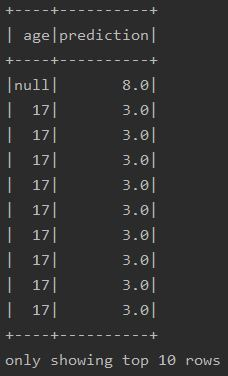
\includegraphics[scale=1]{mllib_naivebayes}
	\caption{Hasil Naive Bayes}
	\label{fig:mllib_naivebayes}
\end{figure}


\subsubsection{K-Means}
\noindent Berikut adalah tahapan eksperimen pada pemodelan K-Means:
\begin{enumerate}
\item Membuat model K-Means menggunakan Spark MLlib
\item Menentukan jumlah cluster (k) untuk pemodelan K-Means.
\item Melakukan pelatihan data pada pemodelan K-Means.
\item Mencari nilai centroid dari masing-masing cluster.
\item Mengembalikan hasil clustering dalam bentuk tabel.

\end{enumerate}	
\begin{lstlisting}[basicstyle=\ttfamily, frame=single,
	columns=fullflexible, keepspaces=true, breaklines=true, label=ls_kepatuhan_1_1_1_logo_sharif_judge, caption=Main method]
	
// KMeans with 8 clusters
val kmeans = new KMeans()
      .setK(8)
      .setFeaturesCol("features")
      .setPredictionCol("prediction")

val kmeansModel = kmeans.fit(result_df)
kmeansModel.clusterCenters.foreach(println)

// Predict model
val predictDf = kmeansModel.transform(result_df)
predictDf.show(10)

\end{lstlisting}

\newpage
\par Hasil dari pemodelan K-Means adalah prediksi jenis cluster berdasarkan sifat dari masing-masing data. Umumnya pada hasil pemodelan K-Means, data-data yang memiliki perbedaan nilai atribut terkecil akan menjadi kelompok cluster yang sama. Pada Gambar \ref{fig:mllib_kmeans}, diketahui bahwa sebuah data yang bernilai (age = 39) memiliki kelompok cluster yang sama (prediction = 5) dengan data lain yang bernilai (age = 38).

\begin{figure}[H]
	\centering
	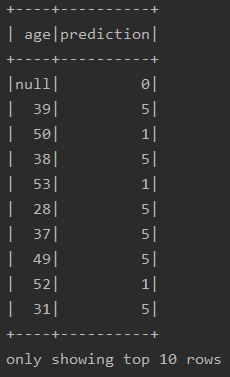
\includegraphics[scale=1]{mllib_kmeans}
	\caption{Hasil K-Means}
	\label{fig:mllib_kmeans}
\end{figure}

\section{Gambaran Umum Perangkat Lunak}
Penelitian ini menghasilkan dua jenis perangkat lunak dengan tujuan yang berbeda satu sama lain, untuk menyelesaikan permasalahan penerapan algorima Greedy K-Member Clustering pada lingkungan big data. Berikut adalah deskripsi perangkat lunak yang akan dibuat:

\begin{enumerate}

\item Perangkat lunak dapat mengimplementasikan algoritma K-Anonymity. Algoritma K-Anonymity yang dimaksud adalah algoritma Greedy K-Member Clustering. Masukan dari perangkat lunak ini adalah dataset Adults dalam format file CSV, tabel atribut quasi-identifier (QID), dan parameter dari algoritma Greedy K-Member Clustering yaitu nilai k dan objek Domain Generalization Hierarchy (DGH). Keluaran dari perangkat lunak ini adalah hasil anonimisasi dari dataset Adults yang disimpan dalam format file CSV.

\item Perangkat lunak dapat membandingkan hasil anonimisasi algoritma K-Anonymity melalui metode data mining yang telah disediakan. Metode data mining yang akan disediakan adalah klasifikasi dengan pemodelan Naive Bayes dan pengelompokan/clustering dengan pemodelan K-Means. Masukan dari perangkat lunak ini adalah dataset Adults dalam format file CSV, baik dataset pernah dilakukan proses anonimisasi maupun dataset asli. Untuk pemodelan K-Means membutuhkan parameter tambahan seperti nilai k dan jenis atribut yang akan diprediksi nilainya. Sedangkan untuk pemodelan Naive Bayes membutuhkan parameter tambahan seperti persentase antara traning dan testing data, jenis atribut yang akan diprediksi nilainya. Keluaran dari perangkat lunak ini untuk pemodelan Naive Bayes dan K-Means memiliki hasil yang sama, yaitu jenis nilai dari atribut yang telah dipilih dan jenis clusternya.

\end{enumerate}

\subsection{Diagram Aktifitas}
Penelitian ini memiliki dua jenis diagram aktivitas,  yaitu diagram aktivitas untuk perangkat lunak anonimisasi data dan diagram aktivitas untuk perangkat lunak analisis data. Tujuan dari membuat dua jenis perangkat lunak antara lain untuk memisahkan perangkat lunak dari fungsionalitas yang berbeda. Fungsionalitas tersebut antara lain melakukan proses anonimisasi data pada dataset dan membandingkan hasil antara dataset asli dengan dataset yang telah dilakukan proses anonimisasi untuk mencari tahu seberapa baik kinerja algoritma Greedy K-Member Clustering untuk mendapatkan hasil yang informatif.

\subsubsection{Perangkat Lunak Anonimisasi Data}
Perangkat lunak ini bertujuan untuk melakukan proses anonimisasi pada dataset Adults menggunakan algoritma K-Anonymity. Diagram aktifitas dapat dilihat pada Gambar \ref{fig:pl_anonimisasi}, berikut adalah tahapan yang terjadi pada perangkat lunak saat melakukan proses anonimisasi data:

\begin{enumerate}

\item Pengguna memberi masukan dalam format file CSV dan beberapa jenis atribut quasi-identifier untuk menjadi tabel input pada proses anonimisasi.

\item Perangkat lunak menampilkan sebagian baris data dari tabel input karena baris data yang akan digunakan pada eksperimen akan berjumlah sangat banyak .

\item Pengguna akan meninjau ulang apakah jumlah kolom yang ditampilkan sudah sesuai dengan jumlah atribut quasi-identifier yang akan dipakai.

\item Penggunakan memberikan parameter tambahan seperti rentang nilai k untuk menentukan jumlah anggota cluster dan objek DGH untuk proses anonimisasi.

\item Perangkat lunak akan melakukan proses anonimisasi dengan bantuan Spark pada tabel input berdasarkan paramater tambahan yang diberikan sebelumnya. 

\item Perangkat lunak mengembalikan seluruh isi log yang dihasilkan selama proses eksekusi Spark berlangsung kepada pengguna untuk deteksi error.

\item Perangkat lunak hanya menampilkan baris data yang berubah akibat proses anonimisasi pada GUI dan hasil keseluruhannya dalam format file CSV.

\item Perangkat lunak mengembalikan nilai information loss pada masing-masing cluster yang terbentuk agar pengguna dapat mencari hasil yang optimal.

\item Pengguna dapat membandingkan hasil anonimisasi antara baris data yang berubah akibat proses anonimisasi dengan baris data yang ada pada tabel asli.

\item Pengguna dapat mengulangi eksperimen untuk mencari nilai k terbaik agar dihasilkan information loss seminimal mungkin pada proses anonimisasi.


 
\end{enumerate}

\subsubsection{Perangkat Lunak Analisis Data}
Perangkat lunak ini bertujuan untuk mencari perbandingan hasil sebelum dan setelah data dilakukan proses anonimisasi dengan metode data mining. Diagram aktifitas dapat dilihat pada Gambar \ref{fig:pl_analisis}, berikut adalah tahapan yang terjadi pada perangkat lunak saat melakukan pemodelan data mining:

\begin{enumerate}

\item Pengguna memberi dua jenis masukan yaitu data asli dan data hasil anonimisasi dalam format file CSV untuk menjadi tabel input pada proses analisis data.

\item Perangkat lunak hanya menampilkan sebagian baris data dari dua jenis tabel input karena input baris data pada eksperimen berjumlah sangat banyak 

\item Pengguna meninjau kembali apakah jumlah kolom yang ditampilkan pada kedua jenis tabel memiliki jumlah kolom atribut yang sama.

\item Pengguna memilih jenis pemodelan data mining yang tersedia pada eksperimen, yaitu klasifikasi dengan Naive Bayes atau pengelompokan/clustering dengan K-Means. 

\item Pengguna mengisi parameter pada pemodelan yang dipilih. Contoh pada K-Means adalah nilai k dan satu jenis atribut. Sedangkan pada Naive Bayes adalah persentase training, testing data dan satu jenis atribut.

\item Perangkat lunak akan melakukan proses pelatihan data pada Spark untuk menemukan klasifikasi/pengelompokan yang sesuai berdasarkan jenis pemodelan yang dipilih.

\item Perangkat lunak mengembalikan seluruh isi log yang dihasilkan selama proses eksekusi Spark berlangsung kepada pengguna untuk deteksi error.

\item Perangkat lunak menampilkan sebagian hasil prediksi cluster untuk masing-masing data dan menyimpan hasil keseluruhannya dalam format file CSV.

\item Pengguna melakukan analisis lebih lanjut terkait pengelompokan dan klasifikasi kelompok data yang terbentuk dari proses pemodelan data mining.
\end{enumerate}

\subsection{Diagram Kelas}
\begin{figure}[H]
	\centering
	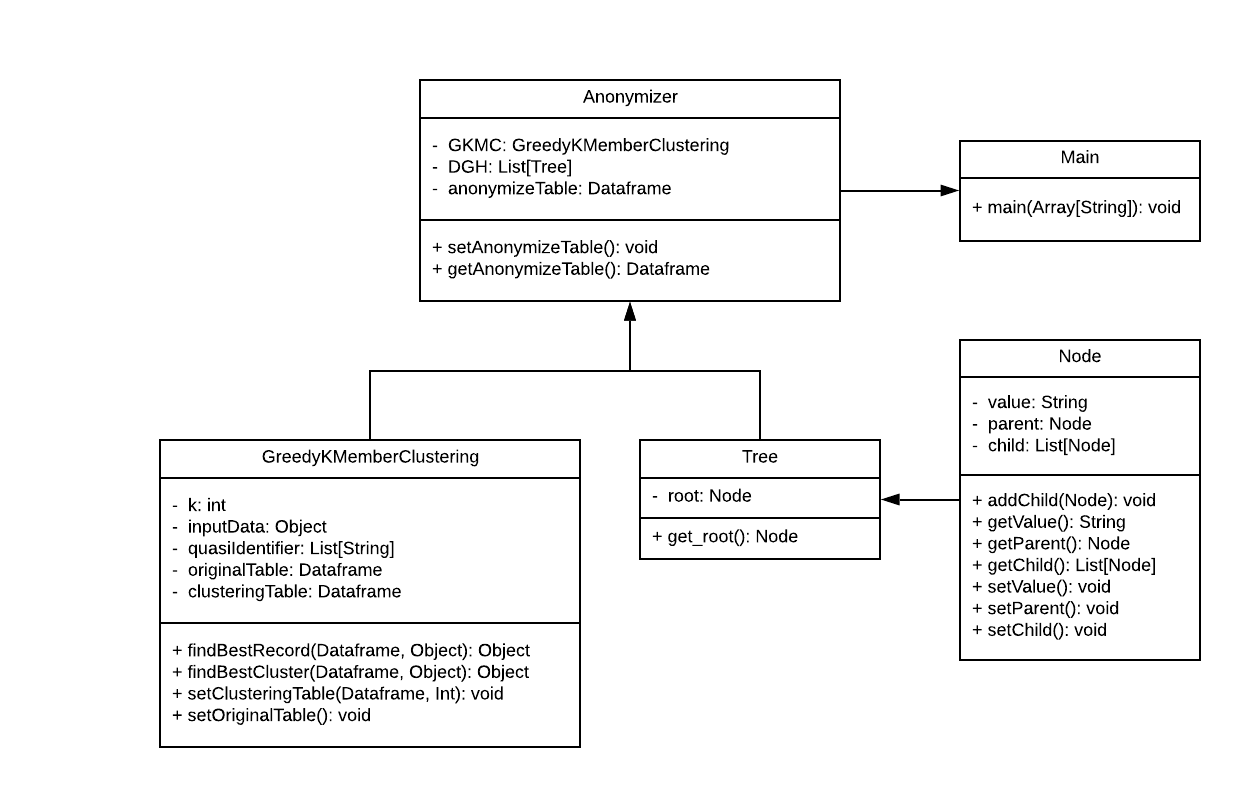
\includegraphics[scale=0.8]{diagram_kelas}
	\caption{Diagram Kelas Anonimisasi Data}
	\label{fig:diagram_kelas}
\end{figure}

Diagram kelas bertujuan untuk menggambarkan keterhubungan antar kelas. Pada penelitian ini digambarkan diagram kelas untuk perangkat lunak anonimisasi data. Karena perangkat lunak analisis data hanya memiliki satu kelas saja, maka keterhubungan antar kelas tidak perlu digambarkan dalam diagram kelas. Gambar 1.1 menggambarkan keterhubungan antar kelas pada perangkat lunak anonimisasi data. Berikut adalah penjelasan lengkap mengenai deskripsi kelas dan method pada perangkat lunak anonimisasi data:

\begin{itemize}
\item Kelas Anonymizer bertujuan untuk melakukan proses anonimisasi setelah data dikelompokan menjadi beberapa cluster. Kelas Anonymizer memiliki 2 jenis variabel, yaitu:

\begin{itemize}

\item GKMC adalah objek dari kelas GreedyKMemberClustering yang berisi tabel hasil pengelompokan data berdasarkan algoritma Greedy K-Member Clustering

\item DGH adalah array 1 dimensi dari objek Tree yang berisi hasil anonimisasi untuk nilai quasi-identifier yang unik agar menjadi nilai yang lebih umum.

\item anonymizeTable adalah array 2 dimensi dari kelas Object untuk menyimpan tabel hasil anonimisasi data.

\end{itemize}

\noindent Kelas Anonymizer memiliki 2 jenis method, yaitu:

\begin{itemize}

\item setAnonymizeTable() bertujuan untuk melakukan proses anonimisasi pada masing-masing baris data yang tergabung dalam sebuah cluster, berdasarkan perbedaan nilai dari beberapa quasi-identifier.

\item getAnonymizeTable() bertujuan untuk mengambil nilai pada atribut anonymizeTable.

\end{itemize}


\item Kelas GreedyKMemberClustering bertujuan untuk melakukan pengelompokan data menjadi beberapa cluster berdasarkan sifat/nilai atribut yang dimiliki oleh masing-masing baris data. Kelas GreedyKMemberClustering memiliki 5 jenis variabel, yaitu:

\begin{itemize}

\item k adalah variabel bertipe Integer untuk membatasi jumlah anggota pada sebuah cluster agar memiliki jumlah yang tetap sebanyak jumlah tertentu.

\item inputData adalah variabel untuk menyimpan seluruh baris data file CSV.

\item quasiIdentifier adalah daftar dari nama-nama kolom yang akan dipilih untuk membuat tabel baru yang digunakan pada proses anonimisasi data

\item originalTable adalah tabel yang menyimpan seluruh baris data pada file CSV berdasarkan jenis kolom yang terpilih pada quasiIdentifier.

\item clusteringTable adalah tabel yang menyimpan hasil pengelompokan baris data dari algoritma Greedy K-Member Clustering.

\end{itemize}

\noindent Kelas GreedyKMemberClustering memiliki 4 jenis method, yaitu:

\begin{itemize}
\item findBestRecord() bertujuan mencari sebuah baris data yang memiliki nilai information loss yang paling minimal dengan baris data lainnya. 

\item findBestCluster() bertujuan mencari sebuah cluster data yang memiliki nilai information loss yang paling minimal dengan cluster lainnya.

\item setClusteringTable() bertujuan mengelompokkan data berdasarkan algoritma Greedy K-Member Clustering dan hasilnya disimpan pada variabel clusteringTable

\item setOriginalTable() bertujuan mengubah hasil pembacaan data input CSV menjadi tabel baru dan hasilnya disimpan pada variabel originalTable

\end{itemize}

\item Kelas Tree bertujuan untuk membuat pohon generalisasi berdasarkan jenis atribut quasi-identfier yang dipilih.

\item Kelas Node bertujuan untuk menyimpan seluruh nilai quasi-identifier yang unik untuk masing-masing baris data.

\item Kelas Main bertujuan untuk membuat tahapan anonimisasi dari awal sampai akhir dengan memanfaatkan pemanggilan method dari masing-masing objek kelas.

\end{itemize}


\begin{figure}[H]
	\centering
	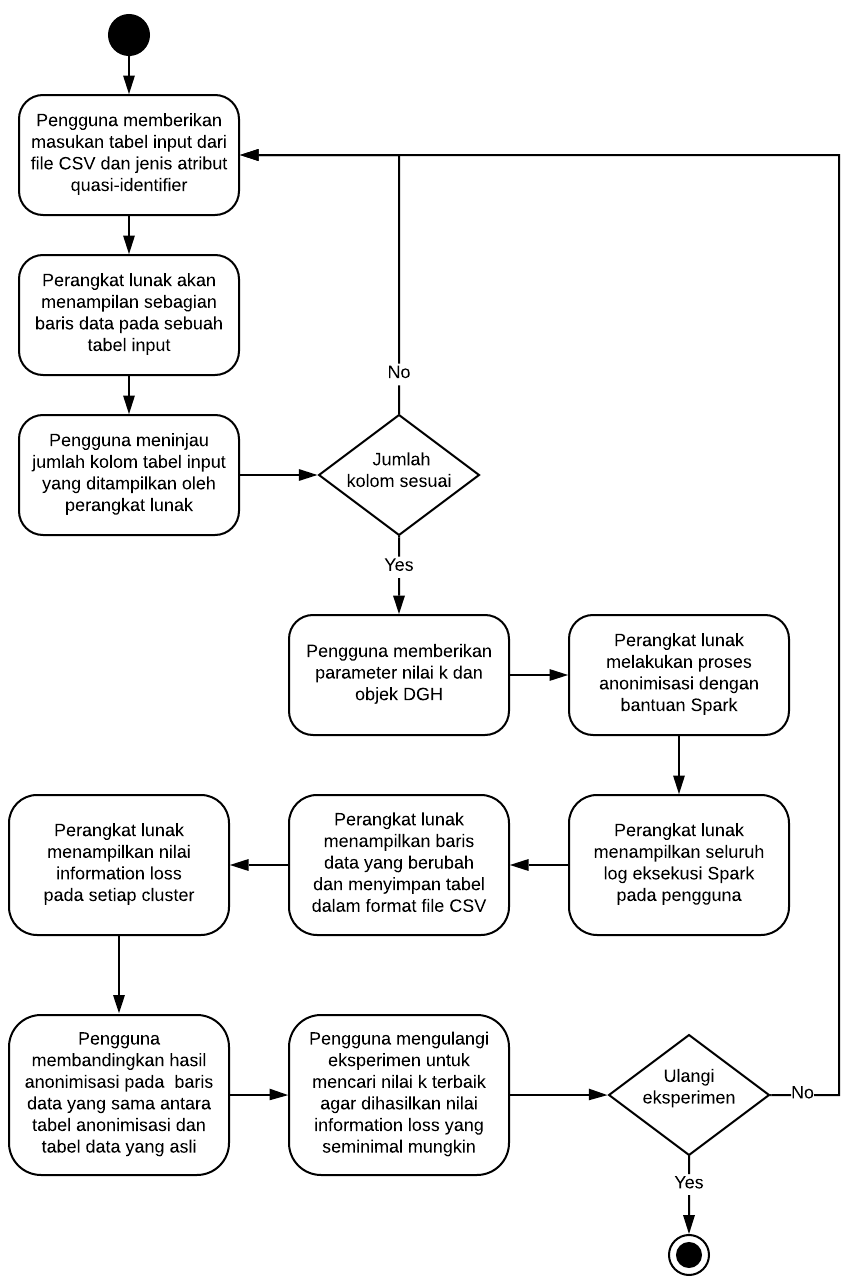
\includegraphics[scale=0.8]{pl_anonimisasi}
	\caption{Diagram Aktifitas Anonimisasi Data}
	\label{fig:pl_anonimisasi}
\end{figure}

\begin{figure}[H]
	\centering
	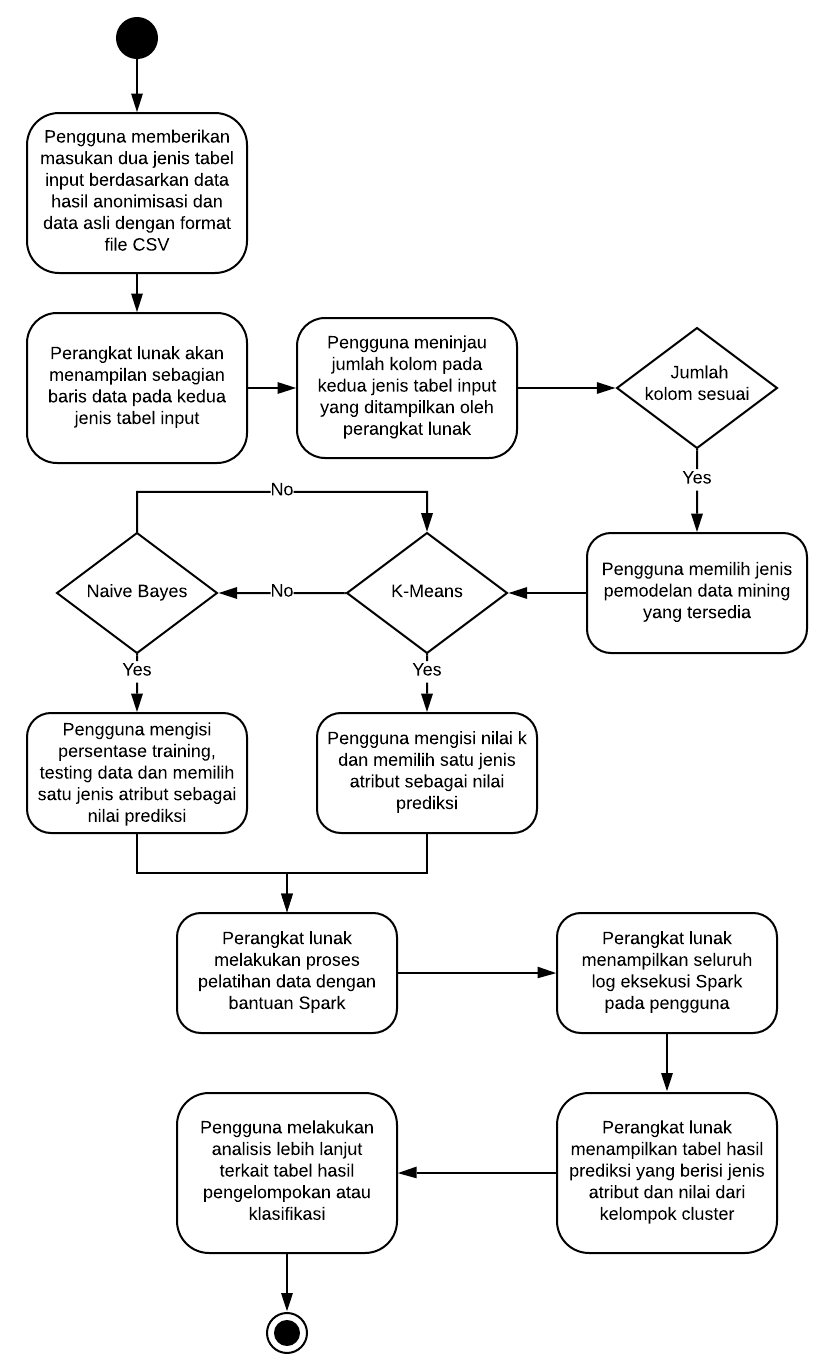
\includegraphics[scale=0.8]{pl_analisis}
	\caption{Diagram Aktifitas Analisis Data}
	\label{fig:pl_analisis}
\end{figure}